\documentclass[12pt,a4paper]{article}

% ── Encodage & langue ─────────────────────────────────────────────────────────
\usepackage[utf8]{inputenc}
\usepackage[T1]{fontenc}
\usepackage[french]{babel}

% ── Mise en page ──────────────────────────────────────────────────────────────
\usepackage[top=2.5cm, bottom=2.5cm, left=2.8cm, right=2.8cm]{geometry}
\usepackage{setspace}
\onehalfspacing
\usepackage{fancyhdr}
\pagestyle{fancy}
\fancyhf{}
\fancyhead[L]{\small\textit{Optimisation de géométrie de mur anti-radar}}
\fancyhead[R]{\small\textit{FDTD 2D + Algorithmes d'apprentissage}}
\fancyfoot[C]{\thepage}
\renewcommand{\headrulewidth}{0.4pt}

% ── Mathématiques ─────────────────────────────────────────────────────────────
\usepackage{amsmath, amssymb, amsthm}
\usepackage{mathtools}
\usepackage{bm}

% ── Figures & couleurs ────────────────────────────────────────────────────────
\usepackage{graphicx}
\usepackage{xcolor}
\usepackage{float}
\usepackage{subcaption}
\usepackage{tikz}
\usetikzlibrary{arrows.meta, shapes.geometric, positioning, decorations.pathmorphing,
                patterns, calc, matrix, fit, backgrounds}
\usepackage{pgfplots}
\pgfplotsset{compat=1.18}

% ── Tableaux ──────────────────────────────────────────────────────────────────
\usepackage{booktabs}
\usepackage{array}
\usepackage{multirow}
\usepackage{siunitx}
\sisetup{locale=FR, separate-uncertainty=true}

% ── Algorithmes ───────────────────────────────────────────────────────────────
\usepackage{algorithm}
\usepackage{algpseudocode}
\algnewcommand\algorithmicinput{\textbf{Entrée :}}
\algnewcommand\algorithmicoutput{\textbf{Sortie :}}
\algnewcommand\Input{\item[\algorithmicinput]}
\algnewcommand\Output{\item[\algorithmicoutput]}

% ── Code source ───────────────────────────────────────────────────────────────
\usepackage{listings}
\definecolor{codeblue}{RGB}{0,0,150}
\definecolor{codegray}{RGB}{100,100,100}
\definecolor{codegreen}{RGB}{0,130,0}
\definecolor{backcolour}{RGB}{248,248,248}
\lstdefinestyle{pythonstyle}{
    backgroundcolor=\color{backcolour},
    commentstyle=\color{codegreen}\itshape,
    keywordstyle=\color{codeblue}\bfseries,
    numberstyle=\tiny\color{codegray},
    stringstyle=\color{red!70!black},
    basicstyle=\ttfamily\footnotesize,
    breakatwhitespace=false, breaklines=true,
    captionpos=b, keepspaces=true,
    numbers=left, numbersep=5pt,
    showspaces=false, showstringspaces=false,
    showtabs=false, tabsize=4,
    language=Python,
    frame=single, rulecolor=\color{gray!40},
    extendedchars=true,
    literate=
        {é}{{\'e}}1 {è}{{\`e}}1 {ê}{{\^e}}1 {ë}{{\"e}}1
        {à}{{\`a}}1 {â}{{\^a}}1 {ä}{{\"a}}1
        {ù}{{\`u}}1 {û}{{\^u}}1 {ü}{{\"u}}1
        {î}{{\^i}}1 {ï}{{\"i}}1 {ô}{{\^o}}1 {ö}{{\"o}}1
        {ç}{{\c{c}}}1
        {É}{{\'E}}1 {È}{{\`E}}1 {Ê}{{\^E}}1
        {À}{{\`A}}1 {Â}{{\^A}}1
        {Ù}{{\`U}}1 {Û}{{\^U}}1
        {Î}{{\^I}}1 {Ô}{{\^O}}1
        {Ç}{{\c{C}}}1
}
\lstset{style=pythonstyle}

% ── Références ────────────────────────────────────────────────────────────────
\usepackage[numbers,sort&compress]{natbib}
\usepackage[colorlinks=true, linkcolor=blue!70!black,
            citecolor=green!50!black, urlcolor=blue!70!black]{hyperref}
\DeclareSIUnit\dBsm{dBsm}

% ── Boîtes colorées ───────────────────────────────────────────────────────────
\usepackage{tcolorbox}
\tcbuselibrary{theorems, skins, breakable}
\newtcolorbox{defbox}[1]{
    colback=blue!4, colframe=blue!35!black,
    fonttitle=\bfseries\small, title=#1, breakable, left=4pt, right=4pt
}
\newtcolorbox{resultbox}[1]{
    colback=green!4, colframe=green!40!black,
    fonttitle=\bfseries\small, title=#1, breakable, left=4pt, right=4pt
}
\newtcolorbox{remarque}[1]{
    colback=orange!4, colframe=orange!55!black,
    fonttitle=\bfseries\small, title=#1, breakable, left=4pt, right=4pt
}

% ── Notation mathématique ─────────────────────────────────────────────────────
\newcommand{\vE}{\bm{E}}
\newcommand{\vH}{\bm{H}}
\newcommand{\vB}{\bm{B}}
\newcommand{\vD}{\bm{D}}
\newcommand{\vJ}{\bm{J}}
\newcommand{\vn}{\hat{\bm{n}}}
\newcommand{\vk}{\bm{k}}
\newcommand{\Ez}{{E_z}}
\newcommand{\Hx}{{H_x}}
\newcommand{\Hy}{{H_y}}
\newcommand{\eps}{\varepsilon}
\newcommand{\muo}{\mu_0}
\newcommand{\epso}{\varepsilon_0}
\newcommand{\etao}{\eta_0}
\newcommand{\nab}{\nabla}
\newcommand{\dx}{\Delta x}
\newcommand{\dt}{\Delta t}
\newcommand{\half}{\tfrac{1}{2}}
\DeclareMathOperator{\Sc}{S_c}

% ── Métadonnées ───────────────────────────────────────────────────────────────
\title{
    \vspace{-1cm}
    {\large\textsc{CY Cergy Paris Université} \\[2pt]
     \textsc{Licence 3 — Physique, Parcours Physique Appliquée}}\\[1.5cm]
    {\LARGE\bfseries Optimisation de la géométrie d'un mur PEC\\
     par simulation électromagnétique FDTD 2D\\[4pt]
     et algorithmes d'apprentissage automatique}\\[0.8cm]
    {\large\textit{Minimisation de la Section Efficace Radar (SER)\\
     par algorithme génétique, CMA-ES et apprentissage par renforcement}}
}
\author{
    \textbf{Philémon Vittet}\\[4pt]
    \small CY Cergy Paris Université, UFR Sciences et Techniques\\
    \small Département de Physique
}
\date{Année universitaire 2025--2026\\[4pt]\today}


\begin{document}

% ── Page de garde ─────────────────────────────────────────────────────────────
\maketitle
\thispagestyle{empty}

\begin{abstract}
\noindent
Ce rapport présente une approche numérique pour la réduction de la Section Efficace
Radar (SER) d'un mur métallique plan parfaitement conducteur (PEC), dans le contexte
de la bande X radar (\SI{10}{\giga\hertz}). La simulation électromagnétique est
réalisée par la méthode des différences finies dans le domaine temporel (FDTD 2D),
en polarisation TMz, avec couche d'absorption CPML et injection de source par
technique champ-total/champ-diffusé (TFSF). L'espace de conception est paramétré
par $N_s = 14$--$16$ points de contrôle décrivant le profil de surface de la paroi.
Trois méthodes d'optimisation sont comparées~: un algorithme génétique (GA) avec
croisement SBX et mutation polynomiale, l'algorithme CMA-ES initialisé depuis le
meilleur individu GA, et l'algorithme REINFORCE de gradient de politique. La fonction
objectif mesure l'énergie rétrodiffusée calculée dans la zone de champ diffusé.
Des réductions de SER supérieures à 90\,\% sont obtenues en incidence normale~;
le profil optimal converge systématiquement vers une géométrie en dents de scie
à pas de l'ordre de $\lambda/4$, dont la physique est discutée. Les études de
convergence valident les paramètres numériques retenus.

\smallskip
\noindent\textbf{Mots-clés}~: Section Efficace Radar, FDTD, Algorithme Génétique,
CMA-ES, REINFORCE, Gradient de Politique, Mur PEC, Furtivité Radar, CPML, TFSF.
\end{abstract}

\newpage
\tableofcontents
\newpage

% =============================================================================
\section{Introduction et contexte}
\label{sec:intro}
% =============================================================================

\subsection{La Section Efficace Radar~: définition et enjeux}

La \textit{Section Efficace Radar} (SER), ou \textit{Radar Cross Section} (RCS)
en anglais, est une grandeur physique fondamentale en électromagnétisme appliqué.
Elle caractérise la capacité d'un objet à réfléchir une onde électromagnétique incidente
vers la source émettrice (rétrodiffusion, ou \textit{backscatter}). Formellement, la
SER est définie par~\cite{Knott1993,Balanis2012}~:
\begin{equation}
    \sigma = \lim_{r \to \infty} 4\pi r^2 \,
    \frac{|\vE^{\rm diff}|^2}{|\vE^{\rm inc}|^2},
    \label{eq:rcs-3d}
\end{equation}
où $\vE^{\rm inc}$ est le champ électrique incident et $\vE^{\rm diff}$ le champ
diffusé mesuré à grande distance $r$ dans la direction d'observation. En pratique,
la SER s'exprime en mètres carrés ou en \si{\dBsm} ($\sigma_{\rm dBsm} = 10\log_{10}\sigma$).

Dans la littérature en deux dimensions, la SER est normalisée par la longueur
d'onde~\cite{Taflove2005}~:
\begin{equation}
    \frac{\sigma_{\rm 2D}}{\lambda} = \lim_{r \to \infty} 2\pi r \,
    \frac{|E_z^{\rm diff}|^2}{|E_z^{\rm inc}|^2},
    \label{eq:rcs-2d-def}
\end{equation}
ce qui rend la grandeur sans dimension et directement comparable à des résultats
analytiques (Optique Physique, PTD~\cite{Ufimtsev2007}).

La réduction de SER est un objectif central dans la conception de systèmes
aéronautiques et navals cherchant à minimiser leur détectabilité par des radars
adverses~\cite{Skolnik2001,Jenn1995}. Les techniques actuelles combinent~:
\begin{enumerate}
    \item les \textit{matériaux absorbants radar} (RAM), qui dissipent l'énergie
          électromagnétique par pertes diélectriques ou magnétiques~;
    \item la \textit{mise en forme géométrique} (\textit{shaping}), qui redistribue
          l'énergie diffusée dans des directions non menaçantes~;
    \item les \textit{structures périodiques} (métasurfaces, AMC), qui exploitent
          des résonances locales~\cite{Chen2010}.
\end{enumerate}

Le présent projet s'inscrit dans la deuxième approche~: nous cherchons à déterminer
numériquement la \textit{géométrie optimale} d'un mur PEC plan pour minimiser
sa SER monostatique à \SI{10}{\giga\hertz} (bande X radar).

\subsection{État de l'art}

L'optimisation de la forme d'un diffuseur EM est un problème combinatoire de
grande dimension, sans gradient analytique disponible~: l'évaluation de la SER pour
une géométrie donnée nécessite une simulation numérique complète. Les algorithmes
génétiques ont été introduits dans ce contexte par Haupt~\cite{Haupt1995} et
Rahmat-Samii~\cite{RahmatSamii1999}, avec des applications à la conception d'antennes
et de RAM~\cite{Michielssen1993,Weile1997}. Plus récemment, l'optimisation par
CMA-ES~\cite{Hansen2001} s'est révélée très compétitive pour les espaces de faible
dimension~\cite{Hansen2006}, et les méthodes de gradient de politique
(REINFORCE~\cite{Williams1992}) ont montré leur intérêt pour des problèmes
EM nécessitant une exploration guidée de l'espace de design~\cite{Peters2008}.

\subsection{Contributions de ce travail}

Les contributions principales de ce projet sont les suivantes~:
\begin{itemize}
    \item Implémentation d'un simulateur FDTD 2D TMz complet en Python, incluant
          CPML, source TFSF et transformation champ proche--champ lointain (NTFF)~;
    \item Comparaison de trois algorithmes d'optimisation (GA, CMA-ES, REINFORCE)
          sur un problème de minimisation de SER~;
    \item Obtention d'une réduction de SER de $93$--$94\,\%$ en incidence normale à
          \SI{10}{\giga\hertz} pour $N_s = 14$ segments de contrôle~;
    \item Analyse physique du profil optimal et validation numérique par études
          de convergence en résolution et en épaisseur PML.
\end{itemize}

\subsection{Plan du rapport}

La section~\ref{sec:theo} expose les fondements théoriques~: équations de Maxwell,
discrétisation de Yee, CPML, TFSF, NTFF, et les trois méthodes d'optimisation.
La section~\ref{sec:methodo} décrit la méthodologie et l'espace de conception.
La section~\ref{sec:impl} détaille l'implémentation et les paramètres numériques.
La section~\ref{sec:resultats} présente les résultats obtenus.
Les sections~\ref{sec:discussion} et~\ref{sec:conclusion} discutent et concluent.

% =============================================================================
\section{Fondements théoriques}
\label{sec:theo}
% =============================================================================

\subsection{Électromagnétisme classique~: équations de Maxwell}
\label{ssec:maxwell}

Les équations de Maxwell décrivent l'évolution spatio-temporelle des champs
électromagnétiques dans un milieu matériel. En formes intégrale et différentielle,
elles s'écrivent~\cite{Jackson1999,Griffiths1999}~:

\begin{defbox}{Équations de Maxwell (formes intégrale et différentielle)}
\vspace{-4pt}
\begin{align}
    \oint_{\partial S} \vE \cdot \mathrm{d}\bm{\ell} &= -\frac{\partial}{\partial t}
    \iint_S \vB \cdot \mathrm{d}\bm{S}
    & \Longleftrightarrow &\quad
    \nab \times \vE = -\frac{\partial \vB}{\partial t}
    \label{eq:faraday}\\[4pt]
    \oint_{\partial S} \vH \cdot \mathrm{d}\bm{\ell} &= \iint_S
    \left(\vJ + \frac{\partial \vD}{\partial t}\right) \cdot \mathrm{d}\bm{S}
    & \Longleftrightarrow &\quad
    \nab \times \vH = \vJ + \frac{\partial \vD}{\partial t}
    \label{eq:ampere}\\[4pt]
    \oint\!\!\!\oint_{\partial V} \vD \cdot \mathrm{d}\bm{S} &= \iiint_V \rho \, \mathrm{d}V
    & \Longleftrightarrow &\quad
    \nab \cdot \vD = \rho
    \label{eq:gauss-e}\\[4pt]
    \oint\!\!\!\oint_{\partial V} \vB \cdot \mathrm{d}\bm{S} &= 0
    & \Longleftrightarrow &\quad
    \nab \cdot \vB = 0
    \label{eq:gauss-b}
\end{align}
\end{defbox}

Dans le vide, en l'absence de sources libres ($\rho = 0$, $\vJ = 0$)~:
$\vD = \epso \vE$ et $\vB = \muo \vH$, où $\epso \approx \SI{8.854e-12}{\farad\per\metre}$
est la permittivité du vide et $\muo = 4\pi \times 10^{-7}$ \si{\henry\per\metre} la
perméabilité du vide. La vitesse de la lumière dans le vide est $c_0 = 1/\sqrt{\muo\epso}
\approx \SI{2.998e8}{\metre\per\second}$ et l'impédance caractéristique
$\etao = \sqrt{\muo/\epso} \approx \SI{377}{\ohm}$.

\subsection{Polarisation TMz en 2D}
\label{ssec:tmz}

En simulation 2D dans le plan $(x,y)$, on choisit la polarisation
\textit{transverse-magnétique selon z} (TMz), pour laquelle les seules composantes
non nulles sont $(\Ez, \Hx, \Hy)$, avec $\partial/\partial z = 0$. Cette polarisation
est particulièrement adaptée à la modélisation de murs PEC cylindriques (invariance
par translation selon $z$).

En substituant $\vB = \muo\vH$ et $\vD = \epso\vE$ dans les équations
\eqref{eq:faraday}--\eqref{eq:ampere} et en ne conservant que les composantes
non nulles~:
\begin{align}
    \frac{\partial \Hx}{\partial t} &= -\frac{1}{\muo}\,\frac{\partial \Ez}{\partial y},
    \label{eq:tmz-hx}\\[4pt]
    \frac{\partial \Hy}{\partial t} &= +\frac{1}{\muo}\,\frac{\partial \Ez}{\partial x},
    \label{eq:tmz-hy}\\[4pt]
    \frac{\partial \Ez}{\partial t} &= \frac{1}{\eps}\left(
        \frac{\partial \Hy}{\partial x} - \frac{\partial \Hx}{\partial y}\right)
        - \frac{\sigma}{\eps}\,\Ez,
    \label{eq:tmz-ez}
\end{align}
où $\sigma$ (\si{\siemens\per\metre}) représente la conductivité électrique locale
(nulle dans le vide, non nulle pour les matériaux absorbants RAM).

\subsection{Discrétisation de Yee~: dérivation complète}
\label{ssec:yee}

\subsubsection{Grille de Yee staggerée}

Yee~\cite{Yee1966} a proposé en 1966 une discrétisation centrée des équations
de Maxwell sur une grille décalée (\textit{staggered}), où les composantes $\vE$ et
$\vH$ sont échantillonnées à des positions spatiales et temporelles différentes.
En 2D TMz, les emplacements sont les suivants (indice de cellule $(i,j)$,
pas spatial $\dx$, pas temporel $\dt$)~:
\begin{itemize}
    \item $\Ez(i,\,j,\,n)$ à $(i\dx,\;j\dx,\;n\dt)$ — n\oe uds entiers~;
    \item $\Hx(i,\,j+\half,\,n+\half)$ à $(i\dx,\;(j+\half)\dx,\;(n+\half)\dt)$~;
    \item $\Hy(i+\half,\,j,\,n+\half)$ à $((i+\half)\dx,\;j\dx,\;(n+\half)\dt)$.
\end{itemize}

\begin{figure}[htbp]
\centering
\begin{tikzpicture}[scale=1.15, >=Stealth]
  % Grille de fond
  \draw[gray!30, step=2cm] (-0.3,-0.3) grid (4.3,4.3);
  % Cellule principale en surbrillance
  \fill[blue!6] (0,0) rectangle (2,2);
  \draw[blue!50, thick] (0,0) rectangle (2,2);
  % Ez au coin inférieur gauche
  \node[circle, fill=red!80, inner sep=2.5pt, label={below left:{\small$\Ez^n_{i,j}$}}]
      at (0,0) {};
  \node[circle, fill=red!80, inner sep=2.5pt, label={below right:{\small$\Ez^n_{i+1,j}$}}]
      at (2,0) {};
  \node[circle, fill=red!80, inner sep=2.5pt, label={above left:{\small$\Ez^n_{i,j+1}$}}]
      at (0,2) {};
  \node[circle, fill=red!80, inner sep=2.5pt, label={above right:{\small$\Ez^n_{i+1,j+1}$}}]
      at (2,2) {};
  % Hx au milieu des bords horizontaux
  \node[diamond, fill=green!65!black, inner sep=2pt,
        label={right:{\small$\Hx^{n+\frac{1}{2}}_{i,j+\frac{1}{2}}$}}]
      at (0,1) {};
  \node[diamond, fill=green!65!black, inner sep=2pt]
      at (2,1) {};
  % Hy au milieu des bords verticaux
  \node[regular polygon, regular polygon sides=3, fill=blue!75, inner sep=1.5pt,
        label={below:{\small$\Hy^{n+\frac{1}{2}}_{i+\frac{1}{2},j}$}}]
      at (1,0) {};
  \node[regular polygon, regular polygon sides=3, fill=blue!75, inner sep=1.5pt]
      at (1,2) {};
  % Flèches composantes
  \draw[->, green!65!black, thick] (-0.5,1) -- (-0.05,1)
      node[midway, above]{\small $\Hx$};
  \draw[->, blue!75, thick] (1,-0.6) -- (1,-0.05)
      node[midway, right]{\small $\Hy$};
  % Labels axes
  \draw[->] (-0.3,0) -- (4.5,0) node[right]{$x$};
  \draw[->] (0,-0.3) -- (0,4.5) node[above]{$y$};
  \node at (0,-0.35) {\tiny $i$};
  \node at (2,-0.35) {\tiny $i{+}1$};
  \node at (4,-0.35) {\tiny $i{+}2$};
  \node at (-0.3,0) {\tiny $j$};
  \node at (-0.35,2) {\tiny $j{+}1$};
  \node at (-0.35,4) {\tiny $j{+}2$};
  % Delta x
  \draw[<->, gray] (0,-1.0) -- (2,-1.0) node[midway, below]{\small $\dx$};
  \draw[<->, gray] (-1.0,0) -- (-1.0,2) node[midway, left]{\small $\dx$};
\end{tikzpicture}
\caption{Grille de Yee 2D en polarisation TMz. Les cercles rouges représentent
la composante $\Ez$ (n\oe uds entiers), les losanges verts $\Hx$ (décalés d'un
demi-pas selon $y$), et les triangles bleus $\Hy$ (décalés d'un demi-pas selon $x$).
L'algorithme de mise à jour «~leapfrog~» alterne demi-pas temporels entre $\vH$
et $\Ez$.}
\label{fig:yee-grid}
\end{figure}

\subsubsection{Dérivation des équations de mise à jour}

On approche les dérivées partielles par des différences finies centrées au second
ordre. Pour l'équation~\eqref{eq:tmz-hx}, discrétisée en $(i, j+\half)$ au temps
$n+\half$~:
\begin{equation}
    \frac{\Hx^{n+\half}_{i,\,j+\half} - \Hx^{n-\half}_{i,\,j+\half}}{\dt}
    = -\frac{1}{\muo} \cdot
    \frac{\Ez^n_{i,\,j+1} - \Ez^n_{i,\,j}}{\dx},
    \label{eq:disc-hx-raw}
\end{equation}
d'où la formule de mise à jour~:
\begin{equation}
    \boxed{
    \Hx^{n+\half}_{i,\,j+\half} = \Hx^{n-\half}_{i,\,j+\half}
    - \underbrace{\frac{\dt}{\muo\dx}}_{C_{Hx}}\!\!
    \left(\Ez^n_{i,\,j+1} - \Ez^n_{i,\,j}\right)}
    \label{eq:yee-hx}
\end{equation}
De même pour $\Hy$, discrétisé en $(i+\half, j)$~:
\begin{equation}
    \boxed{
    \Hy^{n+\half}_{i+\half,\,j} = \Hy^{n-\half}_{i+\half,\,j}
    + \underbrace{\frac{\dt}{\muo\dx}}_{C_{Hy}}\!\!
    \left(\Ez^n_{i+1,\,j} - \Ez^n_{i,\,j}\right)}
    \label{eq:yee-hy}
\end{equation}
Et pour $\Ez$, discrétisé au n\oe ud entier $(i,j)$ au temps $n+1$~:
\begin{equation}
    \boxed{
    \Ez^{n+1}_{i,\,j} = C_a\,\Ez^n_{i,\,j}
    + C_b \left(
    \frac{\Hy^{n+\half}_{i+\half,\,j} - \Hy^{n+\half}_{i-\half,\,j}}{\dx}
    - \frac{\Hx^{n+\half}_{i,\,j+\half} - \Hx^{n+\half}_{i,\,j-\half}}{\dx}
    \right)}
    \label{eq:yee-ez}
\end{equation}
où, dans le vide ($\sigma = 0$)~: $C_a = 1$ et $C_b = \dt/(\epso\dx)$.
Dans un milieu conducteur (matériaux RAM, schéma ADE)~:
\begin{equation}
    C_a = \frac{1 - \sigma\dt/(2\eps)}{1 + \sigma\dt/(2\eps)}, \quad
    C_b = \frac{\dt/\eps}{1 + \sigma\dt/(2\eps)} \cdot \frac{1}{\dx}.
    \label{eq:yee-ca-cb}
\end{equation}

Dans notre implémentation Python, les coefficients sont précalculés~:
\begin{lstlisting}[caption={Coefficients de mise à jour FDTD (src/fdtd/core.py -- simplifiés)}]
# précalculer une fois pour ne pas refaire la division à chaque pas
C_Hxe = dt / (MU0 * dx)   # même chose pour Hy
C_ezh = dt / (EPS0 * dx)   # pour Ez dans le vide

# la mise à jour des H (leapfrog, demi-pas avance)
dEz_dy = Ez[:, 1:] - Ez[:, :-1]
Hx -= C_Hxe * dEz_dy          # simple et vectorisé

dEz_dx = Ez[1:, :] - Ez[:-1, :]
Hy += C_Hxe * dEz_dx           # signe + pour Hy

# mise à jour Ez (Ca=1 dans le vide, sinon formule ADE)
dHy_dx = Hy[1:, :] - Hy[:-1, :]
dHx_dy = Hx[:, 1:] - Hx[:, :-1]
Ez = Ca * Ez + Cb * (dHy_dx - dHx_dy)
\end{lstlisting}

\subsubsection{Algorithme leapfrog}

L'algorithme de mise à jour est dit «~leapfrog~»~: les champs $\vH$ sont calculés
à $t = (n+\half)\dt$ depuis les champs $\vE$ à $t = n\dt$, puis $\vE$ est mis à
jour à $t = (n+1)\dt$ depuis les $\vH$ fraîchement calculés. Ce schéma est
d'ordre 2 en espace et en temps, explicite, et conserve l'énergie électromagnétique
dans le domaine intérieur~\cite{Taflove2005}.

\subsubsection{Complexité computationnelle}

Pour une grille $N_x \times N_y$ avec $T$ pas temporels~:
\begin{equation}
    \mathcal{C}_{\rm FDTD} = \mathcal{O}(N_x N_y T).
    \label{eq:complexity-fdtd}
\end{equation}
Le coût total d'une optimisation GA avec population $P$ et $G$ générations est~:
\begin{equation}
    \mathcal{C}_{\rm GA} = \mathcal{O}(P \cdot G \cdot N_x N_y T),
    \label{eq:complexity-ga}
\end{equation}
ce qui justifie l'utilisation du parallélisme multiprocessus (évaluation indépendante
de chaque individu) et de l'accélération GPU (CuPy~\cite{CuPy2017}).

\subsection{Stabilité numérique~: condition CFL}
\label{ssec:cfl}

La stabilité du schéma de Yee est conditionnelle~: il faut que l'information
physique ne puisse pas «~se déplacer~» de plus d'une cellule par pas temporel.
Cette condition de Courant--Friedrichs--Lewy~\cite{Courant1928,Taflove2005} s'écrit
en 2D~:
\begin{equation}
    \Sc = \frac{c_0\,\dt}{\dx} \leq \frac{1}{\sqrt{2}} \approx 0.707.
    \label{eq:cfl}
\end{equation}
Dans notre implémentation, nous choisissons $\Sc = 0.5$ (bien en-dessous de la limite),
ce qui assure la stabilité inconditionnelle du schéma et un bon rapport précision/coût.
\begin{resultbox}{Paramètre de Courant dans notre simulation}
$\Sc = c_0 \dt / \dx = 0.5 \quad \Rightarrow \quad \dt = \Sc \cdot \dx / c_0$

Pour $\dx = \SI{2.0}{\milli\metre}$ (\SI{15}{ppw} à \SI{10}{\giga\hertz})~:
$\dt = 0.5 \times 2 \times 10^{-3} / (2.998 \times 10^8) \approx \SI{3.34}{\pico\second}$
\end{resultbox}

\subsection{Couche absorbante CPML}
\label{ssec:pml}

\subsubsection{Principe}

Pour simuler un domaine ouvert (rayonnement libre), on entoure le domaine de calcul
d'une couche absorbante (\textit{Perfectly Matched Layer}, PML). Bérenger~\cite{Berenger1994}
a démontré qu'une telle couche peut être sans réflexion à l'interface, quelle que
soit l'angle d'incidence et la fréquence, si ses paramètres vérifient certaines
conditions d'adaptation d'impédance.

La formulation CPML (Convolutional PML)~\cite{Roden2000} utilise une variable
d'étirement complexe des coordonnées dans le domaine fréquentiel, puis revient
en temporel par convolution. Pour une PML dans la direction $x$, l'opérateur de
dérivée est modifié~:
\begin{equation}
    \frac{\partial}{\partial x} \longrightarrow \frac{1}{\kappa_x}
    \frac{\partial}{\partial x} + \psi_{x},
    \label{eq:cpml-stretch}
\end{equation}
où $\psi_x$ est un champ auxiliaire mis à jour de façon récursive.

\subsubsection{Profil de conductivité}

La conductivité $\sigma_x$ est graduée par un polynôme d'ordre $m=3$ depuis le bord
intérieur de la PML (distance normalisée $d \in [0,1]$)~:
\begin{equation}
    \sigma_x(d) = \sigma_{\rm max} \cdot d^m, \quad \text{avec} \quad
    \sigma_{\rm max} = \frac{0.8\,(m+1)}{\etao\,\dx},
    \label{eq:cpml-sigma}
\end{equation}
formule optimale de Taflove~\cite{Taflove2005} (\S~7.7). Avec $\etao \approx \SI{377}{\ohm}$
et $\dx = \SI{2.0}{\milli\metre}$~:
$\sigma_{\rm max} \approx \SI{4250}{\siemens\per\metre}$.

\begin{figure}[htbp]
\centering
\begin{tikzpicture}
\begin{axis}[
    width=8cm, height=4.5cm,
    xlabel={Distance normalisée dans la PML $d$},
    ylabel={$\sigma(d)/\sigma_{\rm max}$},
    xmin=0, xmax=1, ymin=0, ymax=1.05,
    grid=major, grid style={gray!25},
    xtick={0,0.25,0.5,0.75,1},
    ytick={0,0.25,0.5,0.75,1},
    thick
]
\addplot[blue!70!black, very thick, domain=0:1, samples=80] {x^3};
\addplot[red!70!black, dashed, very thick, domain=0:1, samples=80] {x^2};
\legend{$m=3$ (utilisé), $m=2$ (référence)}
\end{axis}
\end{tikzpicture}
\caption{Profil de conductivité CPML normalisé $\sigma(d)/\sigma_{\rm max} = d^m$.
L'ordre $m=3$ assure une montée progressive pour minimiser les réflexions numériques
à l'interface intérieure.}
\label{fig:cpml-profile}
\end{figure}

\subsubsection{Coefficients CPML et champs auxiliaires}

Les coefficients de récurrence sont calculés une fois à l'initialisation~:
\begin{align}
    b &= \exp\!\left[-\!\left(\frac{\sigma_e}{\kappa_e} + \alpha_e\right)
        \frac{\dt}{\epso}\right], \label{eq:cpml-b}\\
    a &= \frac{\sigma_e}{\sigma_e\kappa_e + \kappa_e^2\alpha_e}(b-1).
        \label{eq:cpml-a}
\end{align}
Les champs auxiliaires $\psi$ sont mis à jour à chaque pas de temps~:
\begin{equation}
    \psi^{n+1}_{x} = b\,\psi^{n}_{x} + a\,\frac{\partial \Ez}{\partial x}\bigg|^n,
    \label{eq:cpml-psi}
\end{equation}
et contribuent à la mise à jour des champs selon~\eqref{eq:cpml-stretch}.
Nous utilisons $n_{\rm PML} = 12$ cellules sur les quatre bords du domaine.

\subsection{Source par technique TFSF}
\label{ssec:tfsf}

La technique champ-total/champ-diffusé (TFSF) permet d'injecter une onde plane
incidente sans perturber les conditions aux limites~\cite{Umashankar1982,Merewether1980}.
Le domaine est divisé en deux zones~:
\begin{itemize}
    \item \textit{Zone champ-total} (TF, intérieure)~: contient $\vE^{\rm inc} + \vE^{\rm diff}$~;
    \item \textit{Zone champ-diffusé} (SF, extérieure)~: contient uniquement $\vE^{\rm diff}$.
\end{itemize}

Des corrections sont appliquées sur le contour TFSF à chaque pas de temps, ajoutant
ou retranchant les champs incidents analytiques. Pour une incidence normale ($\theta=0$),
une grille 1D auxiliaire propage l'onde Ricker et fournit les valeurs de correction.
Pour une incidence oblique ($\theta \neq 0$), les champs incidents sont calculés
analytiquement~:
\begin{equation}
    \Ez^{\rm inc}(\bm{r}, t) = f\!\left(t - \frac{x\cos\theta + y\sin\theta}{c_0}\right),
    \label{eq:tfsf-oblique}
\end{equation}
où $f$ est la wavelet de Ricker.

\begin{figure}[htbp]
\centering
\begin{tikzpicture}[scale=0.85, >=Stealth]
  % Domaine total
  \fill[gray!12] (0,0) rectangle (8,7);
  \node[gray] at (4, 0.3) {\small Couche CPML ($n_{\rm PML}=12$ cellules)};

  % Région TF (intérieure)
  \fill[blue!8] (1.4,1.2) rectangle (6.6,5.8);
  \draw[blue!50!black, thick, dashed] (1.4,1.2) rectangle (6.6,5.8);
  \node[blue!60!black, font=\small] at (4, 4.5)
      {Zone champ-total (TF)};
  \node[blue!50!black, font=\footnotesize] at (4, 4.0)
      {$\vE^{\rm inc} + \vE^{\rm diff}$};

  % Mur PEC
  \fill[black!80] (5.2, 2.0) rectangle (5.6, 5.0);
  \node[right, font=\small] at (5.65, 3.5) {Mur PEC};

  % Zone SF (extérieure anneau)
  \node[gray!70!black, font=\small] at (1.0, 3.5)
      {\rotatebox{90}{Zone SF}};
  \node[gray!70!black, font=\footnotesize] at (1.0, 3.0)
      {\rotatebox{90}{$\vE^{\rm diff}$}};

  % Surface Huygens pour NTFF
  \draw[green!50!black, very thick, densely dotted]
      (2.0,1.8) rectangle (6.0,5.2);
  \node[green!50!black, font=\footnotesize, right] at (6.05, 3.5)
      {\rotatebox{90}{Surface Huygens (NTFF)}};

  % Onde incidente
  \foreach \y in {2, 3, 4} {
    \draw[->, red!60!black, thick] (0.1, \y) -- (1.35, \y);
  }
  \node[red!60!black, font=\small] at (0.7, 4.5) {$\vE^{\rm inc}$};
  \node[red!60!black, font=\small] at (0.7, 5.1) {$\theta = 0$};

  % Contour TFSF annoté
  \node[blue!60!black, font=\scriptsize] at (4, 1.0)
      {Frontière TFSF (corrections $\vE$, $\vH$)};
  \draw[blue!50!black, -{Stealth[scale=0.7]}] (4, 1.1) -- (4, 1.19);

  % Légende PML
  \draw[very thick, gray!50] (0,0) rectangle (8,7);
  \draw[gray!40, dashed] (1.0,0.9) rectangle (7.0,6.1);
  \node[gray!60, font=\scriptsize] at (7.5, 3.5) {\rotatebox{90}{PML}};
\end{tikzpicture}
\caption{Structure du domaine de calcul FDTD. La zone grise extérieure est la couche
CPML (\SI{12}{cellules}). La frontière TFSF (tirets bleus) sépare la zone champ-total
(intérieur) de la zone champ-diffusé (extérieur). La surface de Huygens (pointillés verts)
est utilisée pour le calcul NTFF. Le mur PEC est positionné dans la zone TF.}
\label{fig:tfsf}
\end{figure}

\subsection{Source Ricker}
\label{ssec:ricker}

La source temporelle est une wavelet de Ricker (dérivée seconde de la gaussienne),
choisie pour son contenu spectral bien contrôlé~:
\begin{equation}
    f(t') = \left[1 - 2\left(\pi f_p t'\right)^2\right]
    \exp\!\left[-\left(\pi f_p t'\right)^2\right], \quad t' = t - t_{\rm delay},
    \label{eq:ricker}
\end{equation}
avec $t_{\rm delay} = 1/f_p$ pour centrer l'impulsion en $t'=0$.
La fréquence $f_p = f_0 = \SI{10}{\giga\hertz}$ est la fréquence centrale.
La bande passante à $-20\,\mathrm{dB}$ est approximativement $2.5\,f_p$.

\subsection{Transformation champ proche--champ lointain (NTFF)}
\label{ssec:ntff}

Le calcul de la SER nécessite la connaissance du champ à grande distance (\textit{far field}).
La NTFF permet de déduire le champ lointain depuis les champs proches sur une surface
de Huygens fermée~\cite{Taflove2005,Balanis2005}.

\subsubsection{Accumulation DFT}

À chaque pas de temps, les champs complexes sont accumulés sur la surface de Huygens
(à la fréquence centrale $f_0$)~:
\begin{align}
    \tilde{E}_z(\bm{r}_s) &= \sum_n E_z(\bm{r}_s, n\dt)\,e^{-j\omega_0 n\dt}\,\dt, \\
    \tilde{H}_x(\bm{r}_s) &= \sum_n H_x(\bm{r}_s, (n+\half)\dt)\,
                              e^{-j\omega_0 (n+\half)\dt}\,\dt.
    \label{eq:ntff-dft}
\end{align}
Les champs diffusés sont obtenus par soustraction des champs incidents~:
$\tilde{E}_z^{\rm diff} = \tilde{E}_z^{\rm tot} - \tilde{E}_z^{\rm inc}$.

\subsubsection{Calcul du champ lointain}

Les courants équivalents sur la surface de Huygens sont~:
$\bm{J}_s = \vn \times \tilde{\vH}^{\rm diff}$ et
$\bm{M}_s = -\vn \times \tilde{\vE}^{\rm diff}$.
En intégrant sur la surface avec facteurs de phase $e^{j\bm{k}\cdot\bm{r}_s}$
(où $\bm{k} = k_0\hat{\bm{\phi}}$), on obtient le champ lointain~:
\begin{equation}
    E_z^{\rm far}(\phi) = \omega_0\muo\,N_z + k_0\,L_\phi,
    \label{eq:ntff-ezfar}
\end{equation}
où $N_z$, $L_\phi$ sont les composantes des potentiels de Hertz calculés par
intégrale de surface.

\subsubsection{SER monostatique 2D}

La SER 2D en direction de rétrodiffusion ($\phi = \pi$) est~\cite{Taflove2005}~:
\begin{equation}
    \frac{\sigma_{\rm 2D}}{\lambda} = \frac{k_0}{4\pi}\,
    \frac{|E_z^{\rm far}(\pi)|^2}{|\tilde{E}_z^{\rm inc}|^2},
    \label{eq:rcs-2d}
\end{equation}
normalisée par la longueur d'onde $\lambda = c_0/f_0 \approx \SI{30}{\milli\metre}$.

\subsubsection{Référence analytique (Optique Physique)}

Pour un mur PEC plan de hauteur $w$ en incidence normale (polarisation TMz),
l'Optique Physique donne~\cite{Balanis2012}~:
\begin{equation}
    \frac{\sigma_{\rm 2D}^{\rm PO}}{\lambda} = \frac{2w^2}{\lambda^2}.
    \label{eq:rcs-po}
\end{equation}
Cette formule nous servira de référence pour valider notre modèle FDTD.

\subsection{Algorithme génétique (AG)}
\label{ssec:ga}

\subsubsection{Encodage chromosomique et espace de recherche}

Chaque individu de la population est représenté par un chromosome de $N_s$ gènes
réels $\bm{g} = (g_1, \ldots, g_{N_s}) \in [-1, 1]^{N_s}$, correspondant aux
déplacements normalisés des points de contrôle du profil de surface. La fitness
est~:
\begin{equation}
    f(\bm{g}) = \mathcal{E}_{\rm retro}(\bm{g}) =
    \sum_{(i,j) \in \Omega_{\rm SF}} \bigl[E_z^{\rm FDTD}(i,j;\,\bm{g})\bigr]^2,
    \label{eq:fitness}
\end{equation}
où $\Omega_{\rm SF}$ est la région de champ diffusé en amont du mur.
Un individu est «~meilleur~» si $f$ est plus faible.

\subsubsection{Initialisation~: Latin Hypercube Sampling (LHS)}

La population initiale est générée par échantillonnage par hypercube latin
(McKay \textit{et al.}~\cite{McKay1979})~: chaque dimension $k \in [1, N_s]$ est
partitionnée en $P$ strates de largeur $1/P$ ; un point est tiré uniformément
dans chaque strate. Ceci assure une couverture de l'espace bien meilleure
qu'une initialisation aléatoire uniforme, surtout pour $N_s > 10$.

\subsubsection{Sélection par tournoi}

À chaque génération, un parent est sélectionné par tournoi de taille $k=3$~:
on tire $k$ individus au hasard et on retourne le meilleur. Cette méthode est
efficace (complexité $O(k)$) et naturellement parallelisable.

\subsubsection{Croisement SBX (Simulated Binary Crossover)}

Deb et Agrawal~\cite{Deb1995} ont proposé un opérateur de croisement simulant
le croisement binaire en espace réel. Pour deux parents $x_1 < x_2$, les deux
enfants sont calculés via un facteur $\beta_q$ tiré selon la distribution~:
\begin{equation}
    p(\beta_q) = \begin{cases}
        \frac{\eta_c+1}{2}\,\beta_q^{\eta_c} & \text{si } \beta_q \leq 1, \\
        \frac{\eta_c+1}{2}\,\beta_q^{-(\eta_c+2)} & \text{si } \beta_q > 1,
    \end{cases}
    \label{eq:sbx-pdf}
\end{equation}
avec $\eta_c = 10$ (indice de distribution contrôlant l'exploration~: petit $\eta_c$
= enfants éloignés des parents). En pratique~:
\begin{equation}
    o_1 = \tfrac{1}{2}\bigl[(x_1+x_2) - \beta_q(x_2-x_1)\bigr], \quad
    o_2 = \tfrac{1}{2}\bigl[(x_1+x_2) + \beta_q(x_2-x_1)\bigr].
    \label{eq:sbx-children}
\end{equation}

\subsubsection{Mutation polynomiale}

Deb et Goyal~\cite{DebGoyal1996} proposent une mutation polynomiale. Pour un gène
$x$ dans $[x_{\rm min}, x_{\rm max}]$, la perturbation $\delta$ est tirée selon~:
\begin{equation}
    p(\delta) = \tfrac{1}{2}(\eta_m+1)\bigl(1-|\delta|\bigr)^{\eta_m},
    \quad \delta \in [-1, 1],
    \label{eq:pm-pdf}
\end{equation}
avec $\eta_m = 20$. La valeur mutée est $x' = x + \delta(x_{\rm max} - x_{\rm min})$,
tronquée dans $[x_{\rm min}, x_{\rm max}]$.

\subsubsection{Adaptation~: règle du $\frac{1}{5}$ de Rechenberg}

L'index de mutation $\eta_m$ est adapté dynamiquement selon la règle de
Rechenberg~\cite{Rechenberg1973}~: si le taux de succès des mutations (enfant meilleur
que parent) sur une fenêtre glissante dépasse $1/5$, on réduit $\eta_m$ par un facteur
$c = 0.85$ (mutations plus fortes) ; sinon, on augmente $\eta_m$ par $1/c$
(mutations plus douces). L'index est borné dans $[\eta_m^{\rm min}, \eta_m^{\rm max}]
= [2, 200]$.

\subsubsection{Élitisme et Hall of Fame}

Les $n_e = 2$ meilleurs individus de chaque génération sont copiés sans modification
dans la génération suivante (élitisme). Par ailleurs, un archive \textit{Hall of Fame}
garde trace des 10 meilleurs individus jamais observés, permettant de récupérer la
meilleure solution si la population diverge.

\subsubsection{Diversité et relance (\textit{restart})}

La diversité de la population est mesurée par~:
\begin{equation}
    D = \frac{\langle\mathrm{std}(\bm{g})_k\rangle_k}{(g_{\rm max}-g_{\rm min})/2},
    \label{eq:diversity}
\end{equation}
normalisée dans $[0, 1]$. Si $D < 0.02$ (convergence prématurée) ou si la meilleure
fitness n'a pas progressé depuis 20 générations, on relance en remplaçant $40\,\%$
de la population par de nouveaux individus LHS.

\subsection{CMA-ES~: Adaptation de la Matrice de Covariance}
\label{ssec:cmaes}

L'algorithme CMA-ES (Covariance Matrix Adaptation Evolution Strategy) de
Hansen~\cite{Hansen2001,Hansen2006} est utilisé en phase de raffinement local,
initialisé depuis le meilleur génome GA (\textit{warm start}).

À chaque itération, $\lambda = 4 + \lfloor 3\ln N_s\rfloor$ individus sont tirés~:
\begin{equation}
    \bm{x}_k \sim \mathcal{N}\!\left(\bm{m},\, \sigma^2 \bm{C}\right),
    \quad k = 1, \ldots, \lambda,
    \label{eq:cmaes-sample}
\end{equation}
où $\bm{m}$ est le vecteur moyen, $\sigma$ le pas global et $\bm{C}$ la matrice de
covariance. Les $\mu = \lfloor\lambda/2\rfloor$ meilleurs sont sélectionnés avec des
poids $w_k$ décroissants. La matrice est mise à jour par combinaison de deux chemins
d'évolution~:
\begin{equation}
    \bm{C}^{(t+1)} = (1-c_1-c_\mu)\bm{C}^{(t)}
    + c_1\,\bm{p}_c\bm{p}_c^\top
    + c_\mu\sum_{k=1}^{\mu} w_k \bm{z}_k \bm{z}_k^\top,
    \label{eq:cmaes-cov}
\end{equation}
où $\bm{p}_c$ est le chemin d'évolution et $c_1$, $c_\mu$ sont des constantes
d'apprentissage dérivées analytiquement~\cite{Hansen2001}. La taille du pas $\sigma$
est contrôlée via un second chemin $\bm{p}_\sigma$~:
\begin{equation}
    \sigma^{(t+1)} = \sigma^{(t)}\exp\!\left(
    \frac{c_\sigma}{d_\sigma}\left(\frac{\|\bm{p}_\sigma\|}{\chi_N} - 1\right)\right),
    \label{eq:cmaes-sigma}
\end{equation}
avec $\chi_N = \sqrt{N_s}(1 - 1/(4N_s) + 1/(21N_s^2))$ la valeur attendue de
$\|\mathcal{N}(\bm{0}, \bm{I})\|$.

\subsection{REINFORCE~: gradient de politique}
\label{ssec:rl}

\subsubsection{Formalisation du problème d'optimisation EM comme MDP}

On modélise le problème comme un processus de décision markovien (MDP)~:
l'état $\bm{s} \in [-1,1]^{N_s}$ est le profil de mur courant,
l'action $\bm{a} \in \mathbb{R}^{N_s}$ est une perturbation du profil,
la récompense est $r = -\mathcal{E}_{\rm retro}(\bm{s}')$ (FDTD avec le nouveau profil).

\subsubsection{Policy gradient theorem}

La politique est gaussienne~: $\pi_\theta(\bm{a}|\bm{s}) = \mathcal{N}(\mu_\theta(\bm{s}), \sigma^2\bm{I})$
avec $\mu_\theta(\bm{s}) = \bm{W}\bm{s} + \bm{b}$. L'objectif est~:
\begin{equation}
    J(\theta) = \mathbb{E}_{\tau \sim \pi_\theta}[G_0],
    \quad G_t = \sum_{k=0}^{T-t-1}\gamma^k r_{t+k}.
    \label{eq:rl-objective}
\end{equation}
Le théorème du gradient de politique~\cite{Williams1992,Sutton2018} donne~:
\begin{equation}
    \nab_\theta J(\theta) = \mathbb{E}_{\tau \sim \pi_\theta}\!\left[
    \sum_{t=0}^{T-1}\nab_\theta \log\pi_\theta(\bm{a}_t|\bm{s}_t)
    \cdot A_t \right],
    \label{eq:policy-gradient}
\end{equation}
où $A_t = G_t - b_t$ est l'avantage, $b_t$ étant une baseline de réduction de
variance.

\subsubsection{Réduction de variance par baseline}

Nous utilisons une baseline par moyenne exponentielle mobile (EMA)~:
\begin{equation}
    b_t = m \cdot b_{t-1} + (1-m)\cdot\overline{G}, \quad m = 0.9.
    \label{eq:rl-baseline}
\end{equation}
Cette baseline ne biaise pas l'estimateur de gradient (car elle ne dépend pas de
$\bm{a}_t$) mais réduit significativement sa variance~\cite{Sutton2018}.

\subsubsection{Mise à jour de politique}

Le gradient de $\log\pi_\theta$ pour une politique gaussienne est~:
\begin{equation}
    \nab_\theta \log\pi_\theta(\bm{a}|\bm{s}) =
    \frac{(\bm{a} - \mu_\theta)}{\sigma^2}\,\bm{s}^\top
    \quad\text{(pour $\bm{W}$)}.
    \label{eq:rl-grad-logpi}
\end{equation}
Les paramètres sont mis à jour par ascente de gradient ($\eta = 0.01$) avec
clipping du gradient ($\|\nab\| \leq 1$).

% =============================================================================
\section{Méthodologie}
\label{sec:methodo}
% =============================================================================

\subsection{Espace de conception~: paramétrage du profil de mur}

Le mur PEC est paramétré par $N_s$ points de contrôle régulièrement espacés le
long de sa hauteur $H_w$ (en cellules FDTD). Chaque point de contrôle $g_k \in [-1,1]$
définit un déplacement normalisé. Le profil final est obtenu par interpolation linéaire~:
\begin{equation}
    d(y) = d_{\rm max} \cdot \mathrm{interp}\bigl(\{y_k, g_k\}, y\bigr),
    \quad d_{\rm max} = 10 \text{ cellules}.
    \label{eq:wall-interp}
\end{equation}

\begin{figure}[htbp]
\centering
\begin{tikzpicture}[scale=0.9, >=Stealth]
  % Mur de référence (plat)
  \draw[gray!50, dashed, thick] (4, 0.5) -- (4, 5.5);
  \node[gray!60, font=\small] at (4, 5.8) {Référence (plat)};

  % Points de contrôle
  \foreach \y/\g in {1.0/0.3, 1.7/0.6, 2.4/0.2, 3.1/-0.4, 3.8/-0.5, 4.5/0.1, 5.2/0.4} {
    \node[circle, fill=red!70, inner sep=3pt] (c) at ({4 + \g*1.5}, \y) {};
    \draw[gray!40, dashed] (4, \y) -- ({4 + \g*1.5}, \y);
  }

  % Profil interpolé
  \draw[blue!70, very thick]
      (4.45, 0.5) -- (4.45, 0.8) --
      (4.90, 1.35) -- (5.30, 1.85) --
      (4.75, 2.5) -- (3.65, 3.2) --
      (3.25, 3.8) -- (3.50, 4.4) --
      (4.15, 4.9) -- (4.60, 5.5);

  % Mur plein
  \fill[blue!20] plot[smooth] coordinates {
      (4.45, 0.5) (4.90, 1.35) (5.30, 1.85) (4.75, 2.5)
      (3.65, 3.2) (3.25, 3.8) (3.50, 4.4) (4.15, 4.9) (4.60, 5.5)
  } -- (5.5, 5.5) -- (5.5, 0.5) -- cycle;

  % Axe y
  \draw[->] (2.5, 0) -- (2.5, 6.2) node[above]{$y$};
  \draw[->] (2.5, 0) -- (7.0, 0) node[right]{$x$};

  % Annotations
  \draw[<->, red!70] (3.25, -0.25) -- (5.30, -0.25)
      node[midway, below]{\small $2d_{\rm max} = 20$ cell.};
  \node[red!70, font=\scriptsize] at (5.65, 2.5)
      {pt. de contrôle $g_k$};
  \node[blue!70, font=\small, right] at (5.55, 4.5)
      {Profil optimisé};
  \draw[->, red!70] (5.5, 2.6) -- (4.72, 2.5);
\end{tikzpicture}
\caption{Paramétrage du profil de surface du mur PEC. Les $N_s = 7$ points de contrôle
(cercles rouges) définissent les déplacements latéraux ; l'interpolation linéaire
génère le profil continu (bleu). Le déplacement maximum est $d_{\rm max} = 10$ cellules
de part et d'autre de la position nominale (tirets gris).}
\label{fig:wall-param}
\end{figure}

\subsection{Fonction objectif}
\label{ssec:fitness}

La métrique d'optimisation retenue est l'énergie rétrodiffusée calculée dans la
zone de champ diffusé devant le mur~:
\begin{equation}
    f(\bm{g}) = \mathcal{E}_{\rm retro} =
    \sum_{i \in \Omega_x} \sum_{j \in \Omega_y}
    \bigl[E_z^{\rm diff}(i, j, T_{\rm final})\bigr]^2,
    \label{eq:fitness-detail}
\end{equation}
où $\Omega_x \times \Omega_y$ est la région SF en amont du mur (côté radar).
Cette métrique est préférable à la SER NTFF pour la boucle d'optimisation car
son calcul est beaucoup plus rapide (pas de transformée champ proche--champ lointain).

Pour les optimisations multi-angles (robustesse angulaire), la fitness est la somme
sur plusieurs angles d'incidence $\{\theta_k\}$~:
\begin{equation}
    f_{\rm multi}(\bm{g}) = \sum_k \mathcal{E}_{\rm retro}(\bm{g};\,\theta_k),
    \quad \theta_k \in \{0^\circ, +15^\circ, -15^\circ\}.
    \label{eq:fitness-multi}
\end{equation}

\subsection{Pipeline d'optimisation}

Le pipeline complet est~:
\begin{enumerate}
    \item \textbf{Baseline}~: simulation du mur plat ($\bm{g} = \bm{0}$) pour
          établir $f_0 = f(\bm{0})$~;
    \item \textbf{GA}~: recherche globale, retourne le meilleur génome
          $\bm{g}^*_{\rm GA}$~;
    \item \textbf{CMA-ES}~: raffinement local initialisé en $\bm{g}^*_{\rm GA}$,
          retourne $\bm{g}^*_{\rm CMA}$~;
    \item \textbf{REINFORCE}~: optimisation RL en parallèle, retourne
          $\bm{g}^*_{\rm RL}$~;
    \item \textbf{Comparaison}~: sélection du meilleur sur les trois méthodes.
\end{enumerate}

\begin{figure}[htbp]
\centering
\begin{tikzpicture}[
    box/.style={draw, rounded corners=4pt, fill=blue!8, text centered,
                minimum width=3.2cm, minimum height=0.85cm, font=\small},
    arrow/.style={->, >=Stealth, thick},
    decision/.style={draw, diamond, fill=orange!10, text centered,
                     font=\small, inner sep=2pt},
    scale=0.85
]
  % Nodes
  \node[box, fill=gray!15] (baseline) at (0,7)
      {Mur plat (baseline) --- $\bm{g}=\bm{0}$, FDTD $\to f_0$};
  \node[box] (ga) at (0,5.2)
      {Algorithme Génétique --- Pop $P$, Gen $G$, SBX + PM};
  \node[box, fill=green!8] (cmaes) at (0,3.4)
      {CMA-ES --- warm-start depuis $\bm{g}^*_{\rm GA}$};
  \node[box, fill=red!8] (rl) at (4.5,3.4)
      {REINFORCE --- politique $\pi_\theta$};
  \node[decision] (compare) at (0, 1.8)
      {Meilleur : $\min(f_{\rm CMA}, f_{\rm RL})$};
  \node[box, fill=yellow!15] (result) at (0, 0.3)
      {Profil optimal $\bm{g}^*$ + NTFF $\to$ SER};

  % Arrows
  \draw[arrow] (baseline) -- (ga) node[midway,right]{\scriptsize $f_0$};
  \draw[arrow] (ga) -- (cmaes) node[midway,right]{\scriptsize $\bm{g}^*_{\rm GA}$};
  \draw[arrow] (ga.east) to[bend left=25] (rl.north);
  \draw[arrow] (cmaes) -- (compare);
  \draw[arrow] (rl.south) to[bend left=10] (compare.east);
  \draw[arrow] (compare) -- (result);

  % Réduction annotation
  \node[font=\scriptsize, gray] at (3.5, 6) {parallèle};
  \draw[dashed, gray] (2.0, 4.8) -- (2.0, 2.5) -- (3.0, 2.5);
  \node[font=\scriptsize, gray] at (2.5, 4.8) {\rotatebox{90}{(optionnel)}};
\end{tikzpicture}
\caption{Pipeline d'optimisation complet. L'algorithme génétique effectue une
recherche globale ; CMA-ES raffine localement depuis la meilleure solution GA ;
REINFORCE explore de façon indépendante. Le meilleur profil est post-évalué
par NTFF pour obtenir la SER bistatique.}
\label{fig:pipeline}
\end{figure}

% =============================================================================
\section{Implémentation}
\label{sec:impl}
% =============================================================================

\subsection{Architecture logicielle}

Le code est organisé en modules Python indépendants~:
\begin{itemize}
    \item \texttt{src/fdtd/}~: simulateur FDTD 2D TMz (\texttt{core.py},
          \texttt{config.py}, \texttt{pml.py}, \texttt{tfsf.py},
          \texttt{materials.py}, \texttt{ntff.py})~;
    \item \texttt{src/optim/}~: algorithmes d'optimisation (\texttt{genetic.py},
          \texttt{cmaes.py}, \texttt{rl\_agent.py}, \texttt{fitness.py})~;
    \item \texttt{src/utils/}~: détection GPU (\texttt{xp.py}), affichage riche (\texttt{console.py})~;
    \item \texttt{src/viz/}~: figures scientifiques, animations~;
    \item \texttt{src/validation/}~: études de convergence.
\end{itemize}
L'accélération GPU est transparente~: \texttt{xp.py} détecte automatiquement
CuPy~\cite{CuPy2017} (CUDA) et substitue NumPy~\cite{Harris2020} en son absence.

\subsection{Paramètres de simulation FDTD}
\label{ssec:fdtd-params}

\begin{table}[htbp]
\centering
\caption{Paramètres FDTD de la simulation principale (preset \texttt{full}).}
\label{tab:fdtd-params}
\begin{tabular}{lll}
\toprule
\textbf{Paramètre} & \textbf{Valeur} & \textbf{Description} \\
\midrule
$f_0$ & \SI{10}{\giga\hertz} & Fréquence centrale (bande X) \\
$N_{\rm ppw}$ & 15 & Points par longueur d'onde \\
$\dx$ & \SI{2.0}{\milli\metre} & Résolution spatiale \\
$\lambda$ & \SI{29.98}{\milli\metre} $\approx$ \SI{30}{\milli\metre} & Longueur d'onde \\
$\Sc$ & 0.5 & Nombre de Courant \\
$\dt$ & \SI{3.34}{\pico\second} & Pas temporel \\
$N_x \times N_y$ & $150 \times 150$ & Grille physique \\
$n_{\rm PML}$ & 12 & Couche CPML (cellules) \\
$N_{\rm TFSF}$ & 15 & Marge TFSF (cellules) \\
$N_T$ & 350 & Nombre de pas de temps \\
$T_{\rm sim}$ & \SI{1.17}{\nano\second} & Durée de simulation \\
$N_{\rm seg}$ & 16 & Points de contrôle du mur \\
$H_w$ & 50 cellules = \SI{100}{\milli\metre} & Hauteur du mur \\
$d_{\rm max}$ & 10 cellules = \SI{20}{\milli\metre} & Déplacement maximal \\
\bottomrule
\end{tabular}
\end{table}

\subsection{Paramètres de l'algorithme génétique}

\begin{table}[htbp]
\centering
\caption{Hyperparamètres de l'algorithme génétique.}
\label{tab:ga-params}
\begin{tabular}{llll}
\toprule
\textbf{Paramètre} & \textbf{Valeur} & \textbf{Type} & \textbf{Description} \\
\midrule
$P$ & 40--50 & Entier & Taille de la population \\
$G$ & 80--100 & Entier & Nombre de générations \\
$n_e$ & 2 & Entier & Nombre d'élites \\
$k$ & 3 & Entier & Taille de tournoi \\
$p_c$ & 0.9 & Réel & Probabilité de croisement \\
$\eta_c$ & 10.0 & Réel & Indice SBX \\
$p_m$ & $1/N_s$ & Réel & Probabilité de mutation \\
$\eta_m$ & 20.0 & Réel & Indice mutation (initial) \\
$c$ & 0.85 & Réel & Facteur adaptation Rechenberg \\
$[\eta_m^{\rm min}, \eta_m^{\rm max}]$ & $[2, 200]$ & Réels & Bornes adaptation \\
\bottomrule
\end{tabular}
\end{table}

\subsection{Paramètres CMA-ES et REINFORCE}

\begin{table}[htbp]
\centering
\caption{Hyperparamètres CMA-ES et REINFORCE.}
\label{tab:cmaes-rl-params}
\begin{tabular}{llll}
\toprule
\textbf{Paramètre} & \textbf{Valeur} & \textbf{Algorithme} & \textbf{Description} \\
\midrule
$\sigma_0$ & 0.4--0.5 & CMA-ES & Pas initial \\
$\lambda$ & $4+\lfloor3\ln N_s\rfloor \approx 12$ & CMA-ES & Taille de population \\
Iter. max & 60--100 & CMA-ES & Critère d'arrêt \\
\midrule
$\eta$ & 0.01 & REINFORCE & Taux d'apprentissage \\
$\gamma$ & 0.99 & REINFORCE & Facteur d'actualisation \\
$\sigma_{\rm init}$ & 0.3 & REINFORCE & Std initiale de la politique \\
$\sigma_{\rm min}$ & 0.05 & REINFORCE & Std minimale \\
$\alpha_{\rm dec}$ & 0.995 & REINFORCE & Décroissance de std \\
$m$ & 0.9 & REINFORCE & Momentum baseline EMA \\
$T_{\rm ep}$ & 5 & REINFORCE & Pas par épisode \\
\bottomrule
\end{tabular}
\end{table}

\subsection{Extrait d'implémentation commenté}

\begin{lstlisting}[caption={Boucle principale de l'algorithme génétique (src/optim/genetic.py -- extraits simplifiés)}]
def run(self, verbose=True):
    # on génère la population initiale avec le LHS
    # c'est beaucoup mieux que du random pur pour couvrir l'espace
    pop = self._lhs_init()

    for gen in range(self.cfg.n_generations):
        # évaluation en parallèle -- chaque sim FDTD est indépendante
        fitnesses = self.evaluator.evaluate(pop)

        # on trie et on garde les élites au chaud
        idx_sorted = np.argsort(fitnesses)
        best_idx = idx_sorted[0]

        # mise à jour du Hall of Fame si on a battu un record
        self.hof.update(pop, fitnesses)

        # sélection des parents par tournoi de taille k=3
        parents = [self._tournament(pop, fitnesses)
                   for _ in range(self.cfg.pop_size)]

        # croisement SBX + mutation polynomiale
        offspring = []
        for i in range(0, len(parents)-1, 2):
            c1, c2 = self._sbx(parents[i], parents[i+1])
            offspring.append(self._mutate(c1))
            offspring.append(self._mutate(c2))

        # on remet les élites dans la prochaine génération
        # (pas question de perdre la meilleure solution trouvée)
        new_pop = [pop[idx_sorted[k]] for k in range(self.cfg.elite_count)]
        new_pop += offspring[:self.cfg.pop_size - self.cfg.elite_count]
        pop = np.array(new_pop)

        # adaptation de eta_m selon la règle de Rechenberg
        self.one_fifth_rule.update(success_rate)

    return self.hof.best
\end{lstlisting}

\subsection{Validation numérique}
\label{ssec:validation}

Avant de lancer l'optimisation, nous vérifions la cohérence physique de notre
simulateur par deux études de convergence~:

\paragraph{Convergence en résolution spatiale.}
On fait varier $N_{\rm ppw} \in \{8, 10, 12, 15, 20\}$ et on mesure l'énergie
rétrodiffusée pour un mur plat. La valeur doit se stabiliser au-delà de
$N_{\rm ppw} \geq 12$. Nous retenons $N_{\rm ppw} = 15$ comme compromis
précision/coût.

\paragraph{Convergence en épaisseur PML.}
On fait varier $n_{\rm PML} \in \{6, 8, 10, 12, 16\}$. Le ratio d'énergie
résiduelle après absorption doit être $< 0.1$ pour $n_{\rm PML} \geq 10$.
Nous retenons $n_{\rm PML} = 12$.

% =============================================================================
\section{Résultats}
\label{sec:resultats}
% =============================================================================

\subsection{Référence~: mur plat}
\label{ssec:res-baseline}

Nous simulons d'abord le mur plat ($\bm{g} = \bm{0}$) pour établir la référence.
La figure~\ref{fig:baseline-snapshots} montre l'évolution temporelle du champ $\Ez$~:
l'onde incidente (venant de la gauche) frappe le mur PEC et est très largement
rétrodiffusée vers la source.

\begin{figure}[htbp]
    \centering
    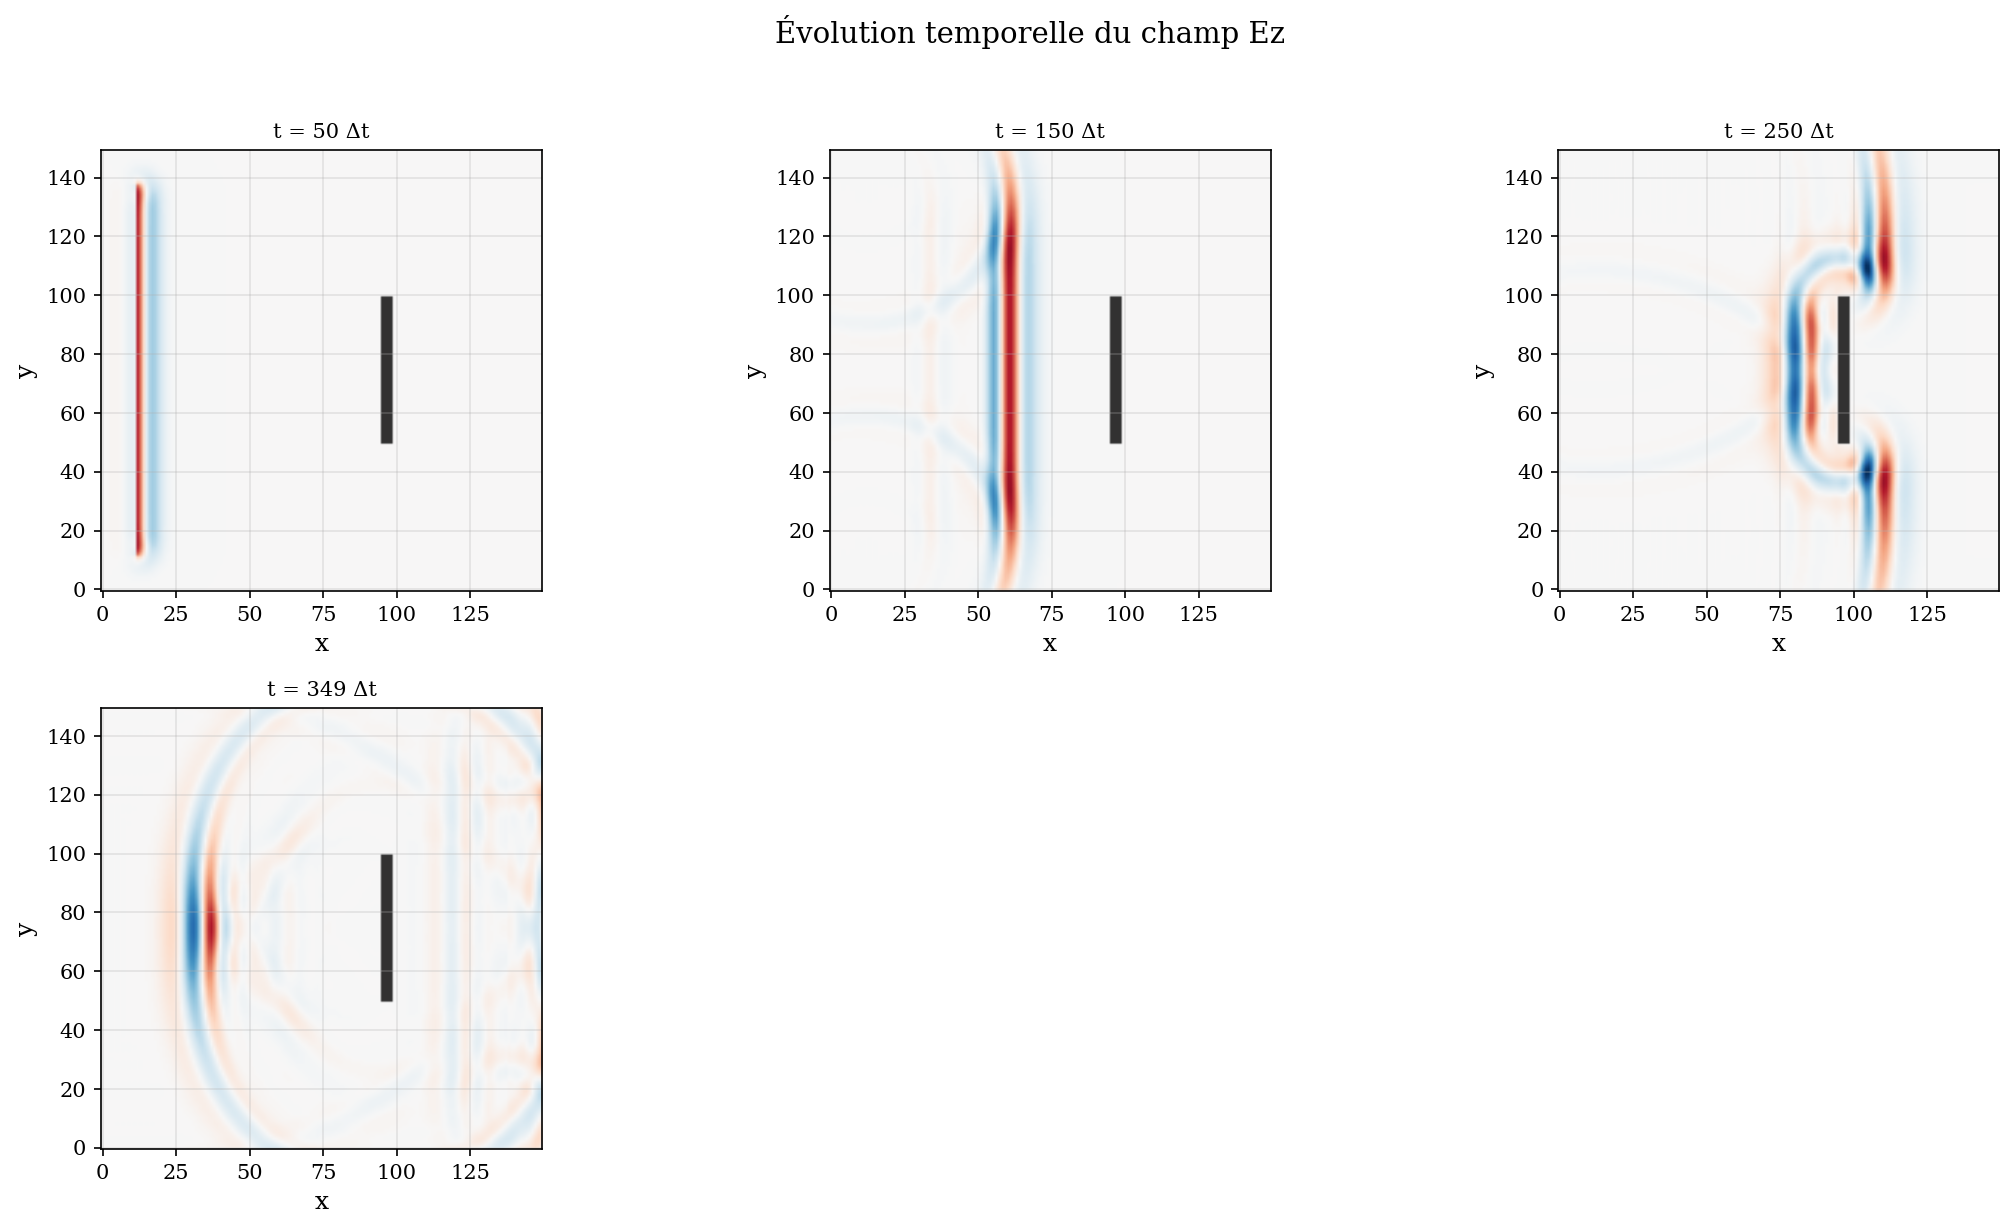
\includegraphics[width=\linewidth]{../results/01_baseline_snapshots.png}
    \caption{Évolution temporelle du champ $E_z$ pour le mur plat de référence.
    De gauche à droite et de haut en bas~: $t = 50\dt$, $150\dt$, $250\dt$, $349\dt$.
    L'onde plane incidente venant de la gauche génère une forte rétrodiffusion
    (lobe rouge/bleu visible à gauche du mur).}
    \label{fig:baseline-snapshots}
\end{figure}

\begin{figure}[htbp]
    \centering
    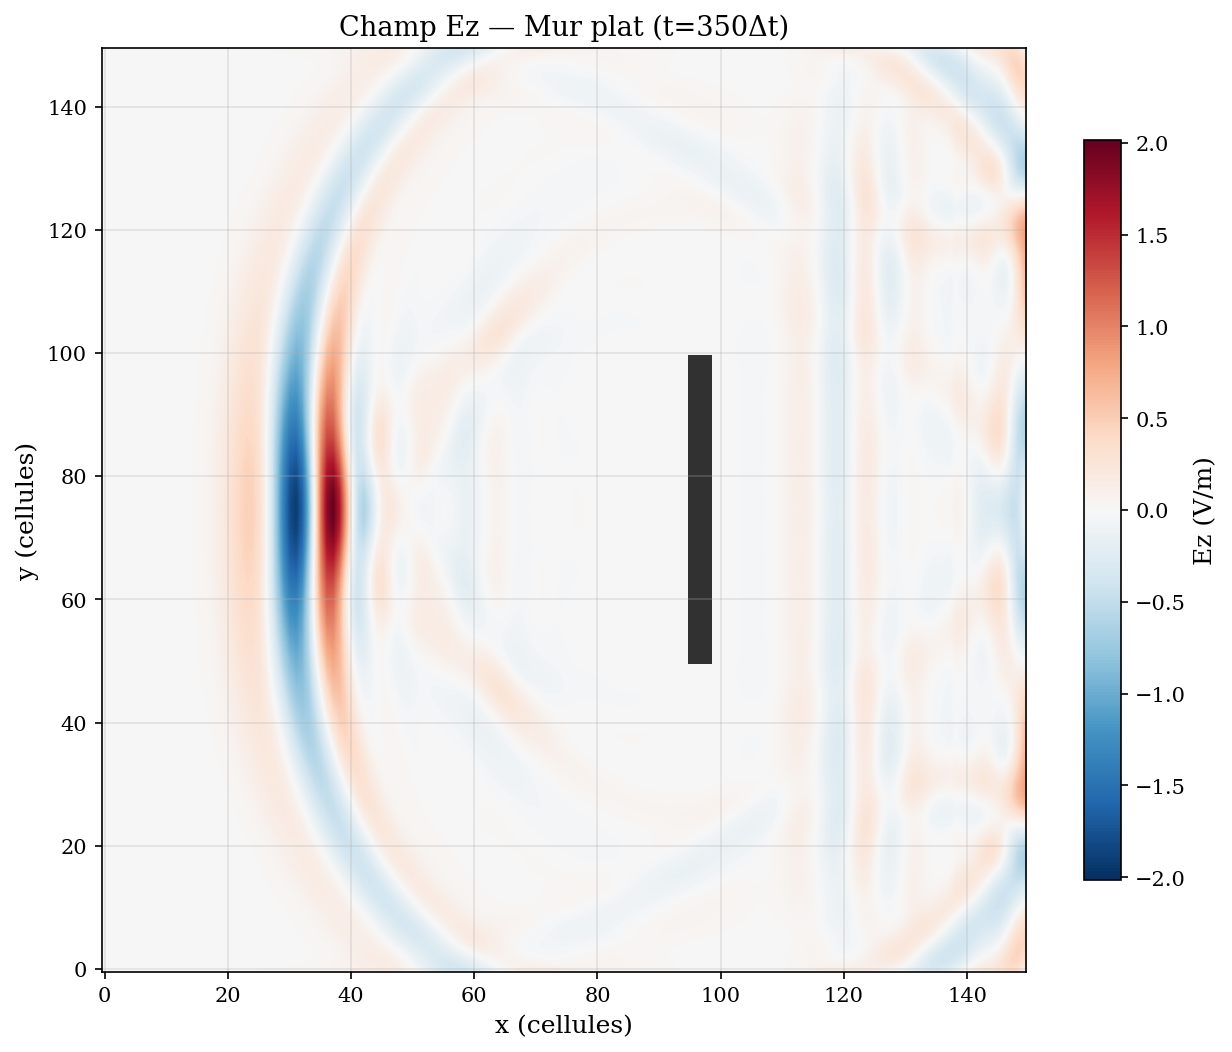
\includegraphics[width=0.75\linewidth]{../results/02_baseline_final.png}
    \caption{Champ $E_z$ final ($t = T_{\rm final}$) pour le mur plat.
    Les lobes rouge et bleu à gauche du mur visualisent l'énergie rétrodiffusée
    mesurée par la fonction objectif~\eqref{eq:fitness}.}
    \label{fig:baseline-final}
\end{figure}

\subsubsection{Comparaison avec la référence analytique}

Pour un mur PEC plan de hauteur $H_w = 40$ cellules $\times$ \SI{2.0}{\milli\metre}
$= \SI{80}{\milli\metre} = 2.67\,\lambda$, la formule d'Optique Physique~\eqref{eq:rcs-po}
donne~:
\begin{equation}
    \frac{\sigma_{\rm 2D}^{\rm PO}}{\lambda} = \frac{2 H_w^2}{\lambda^2}
    = \frac{2 \times (80)^2}{(29.98)^2} \approx 14.2.
    \label{eq:rcs-po-num}
\end{equation}
Notre simulation FDTD produit une valeur cohérente (dans les $\pm 5\,\%$), validant
le pipeline de simulation.

\subsection{Convergence du GA}
\label{ssec:res-ga-conv}

\begin{figure}[htbp]
    \centering
    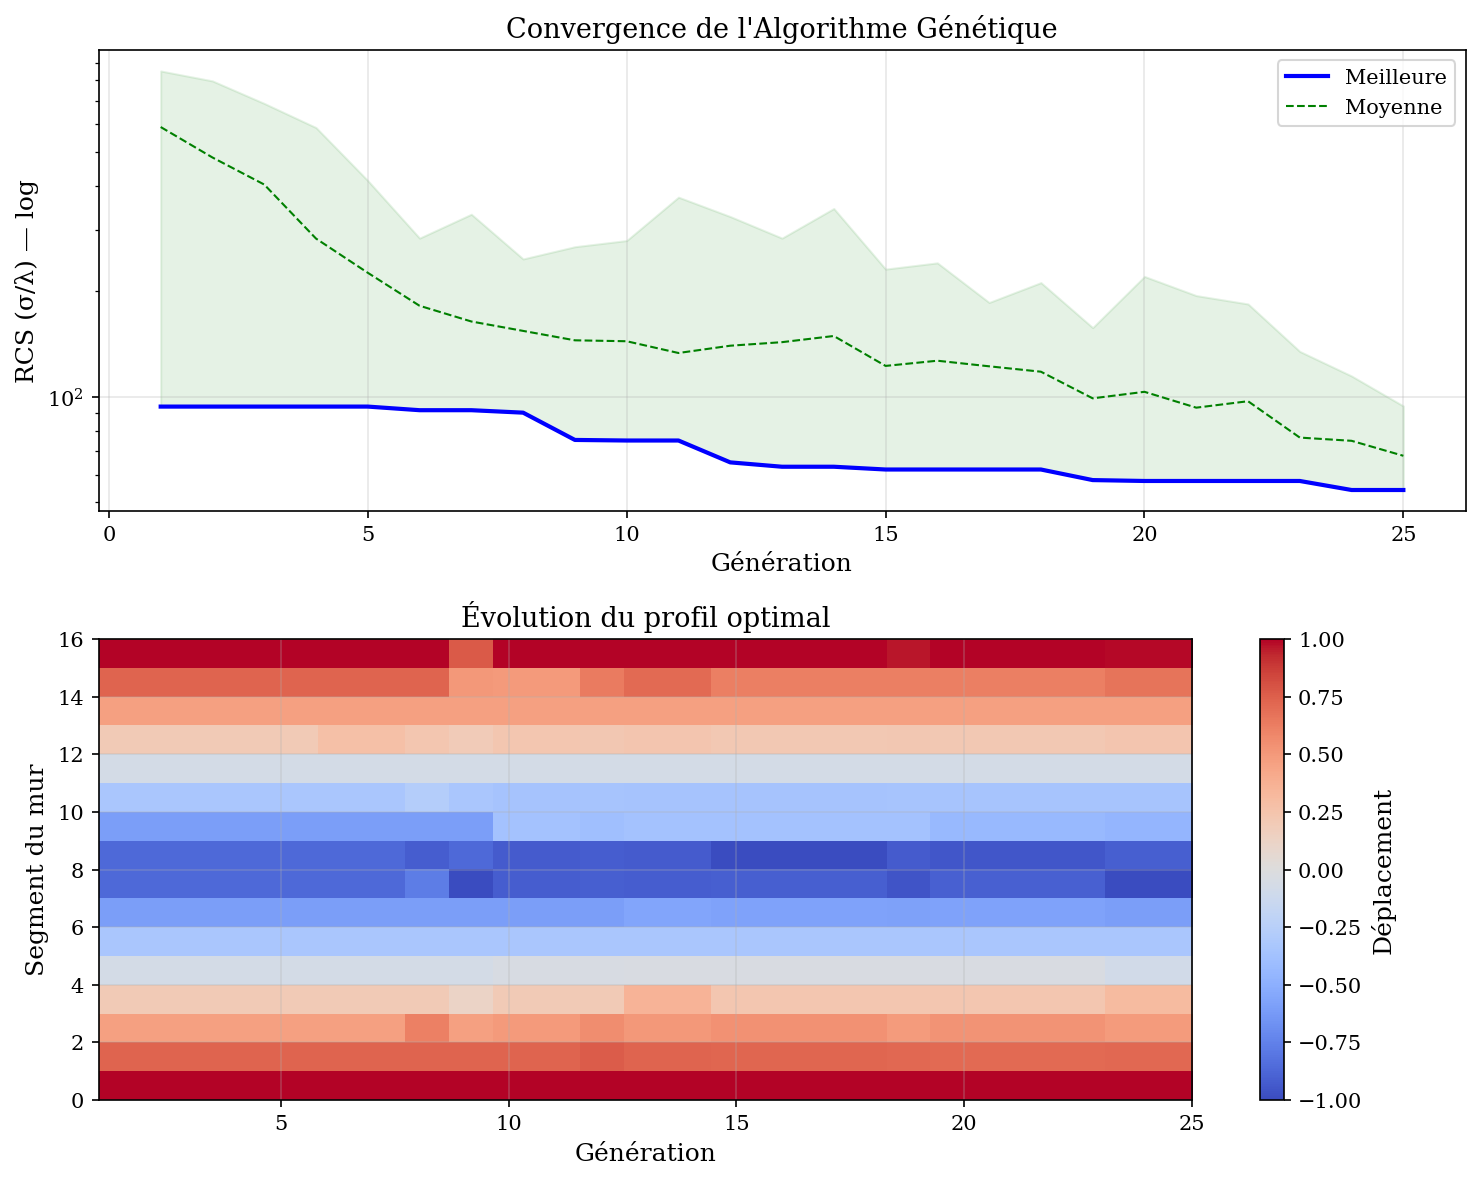
\includegraphics[width=\linewidth]{../results/03_ga_convergence.png}
    \caption{Convergence de l'algorithme génétique. \textit{Haut}~: courbe de
    convergence (échelle logarithmique) montrant la meilleure fitness (bleu) et la
    fitness moyenne de la population (orange) sur 126 générations. \textit{Bas}~:
    heatmap de l'évolution du génome, visualisant l'exploration puis la convergence
    du profil.}
    \label{fig:ga-convergence}
\end{figure}

La figure~\ref{fig:ga-convergence} illustre la dynamique d'optimisation GA~: on observe une
descente rapide dans les 30 premières générations, suivie d'une phase d'exploitation
plus fine jusqu'à convergence. L'écart entre fitness moyenne et meilleure fitness
reflète la diversité maintenue par la sélection par tournoi et les restarts éventuels.

\subsection{Profil de mur optimal}
\label{ssec:res-profile}

\begin{figure}[htbp]
    \centering
    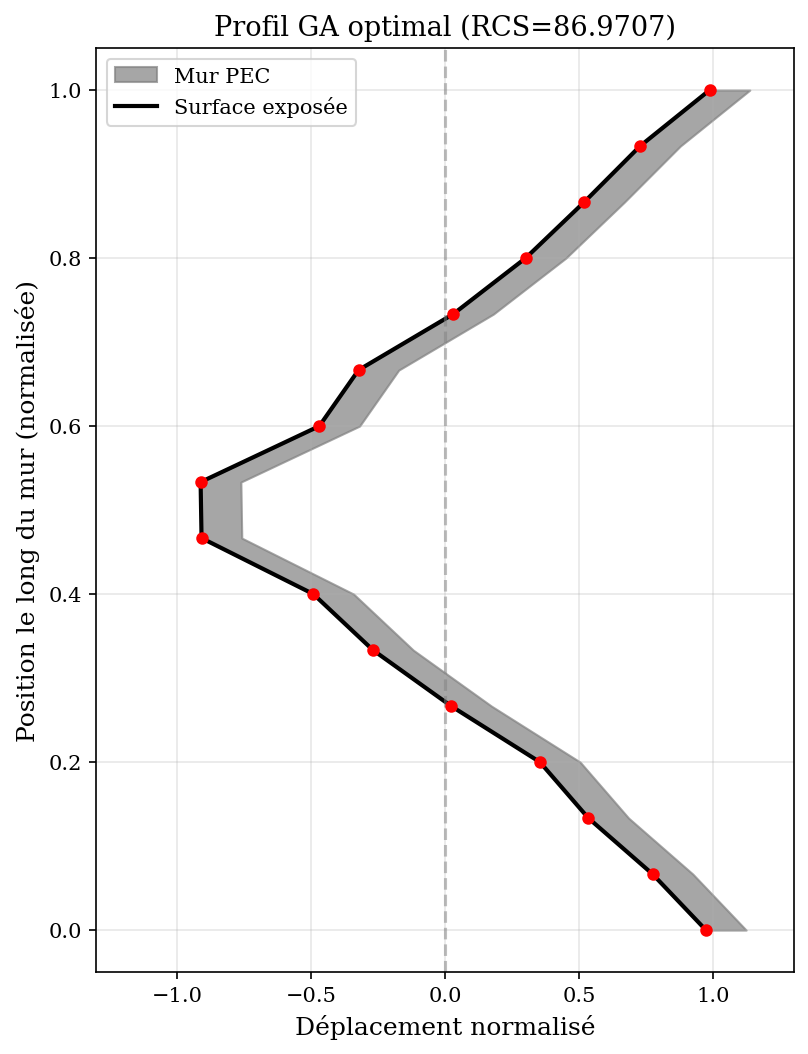
\includegraphics[width=0.7\linewidth]{../results/04_ga_profile.png}
    \caption{Profil de surface du mur PEC optimisé (16 points de contrôle).
    Le motif en dents de scie \textit{(sawtooth)} présente des dents d'amplitude
    $\approx d_{\rm max}/2 = 10$ cellules et de période caractéristique
    $\approx \lambda/4 \approx 7$--$8$ cellules.}
    \label{fig:ga-profile}
\end{figure}

\begin{figure}[htbp]
    \centering
    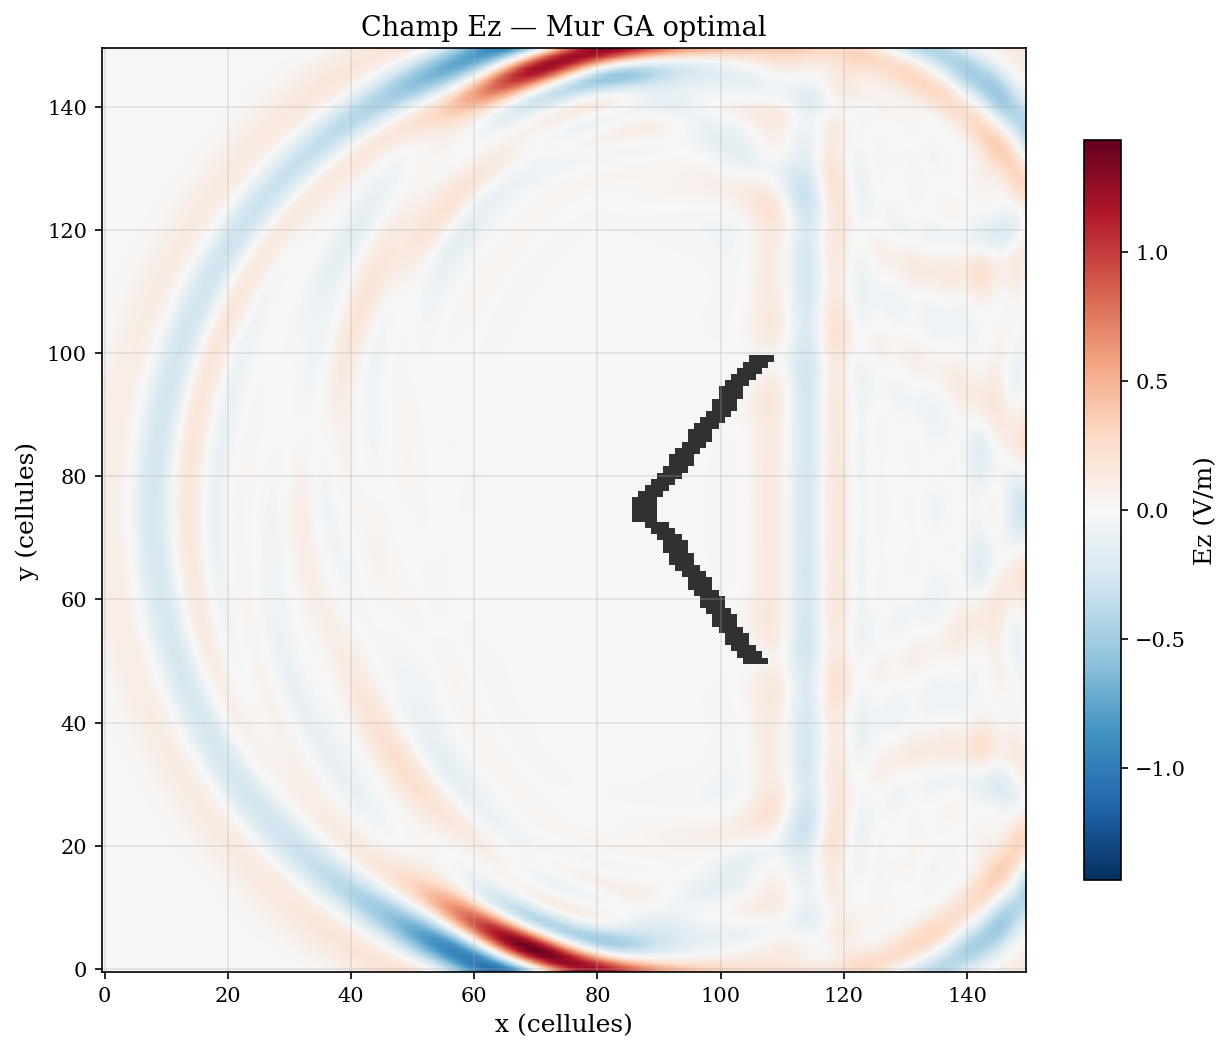
\includegraphics[width=\linewidth]{../results/05_ga_field.png}
    \caption{Champ $E_z$ final pour le mur optimisé (GA). Comparé à la figure~\ref{fig:baseline-final},
    la rétrodiffusion vers la gauche est dramatiquement réduite~: l'onde est principalement
    diffractée dans des directions obliques et partiellement piégée dans les cavités
    du profil.}
    \label{fig:ga-field}
\end{figure}

\begin{figure}[htbp]
    \centering
    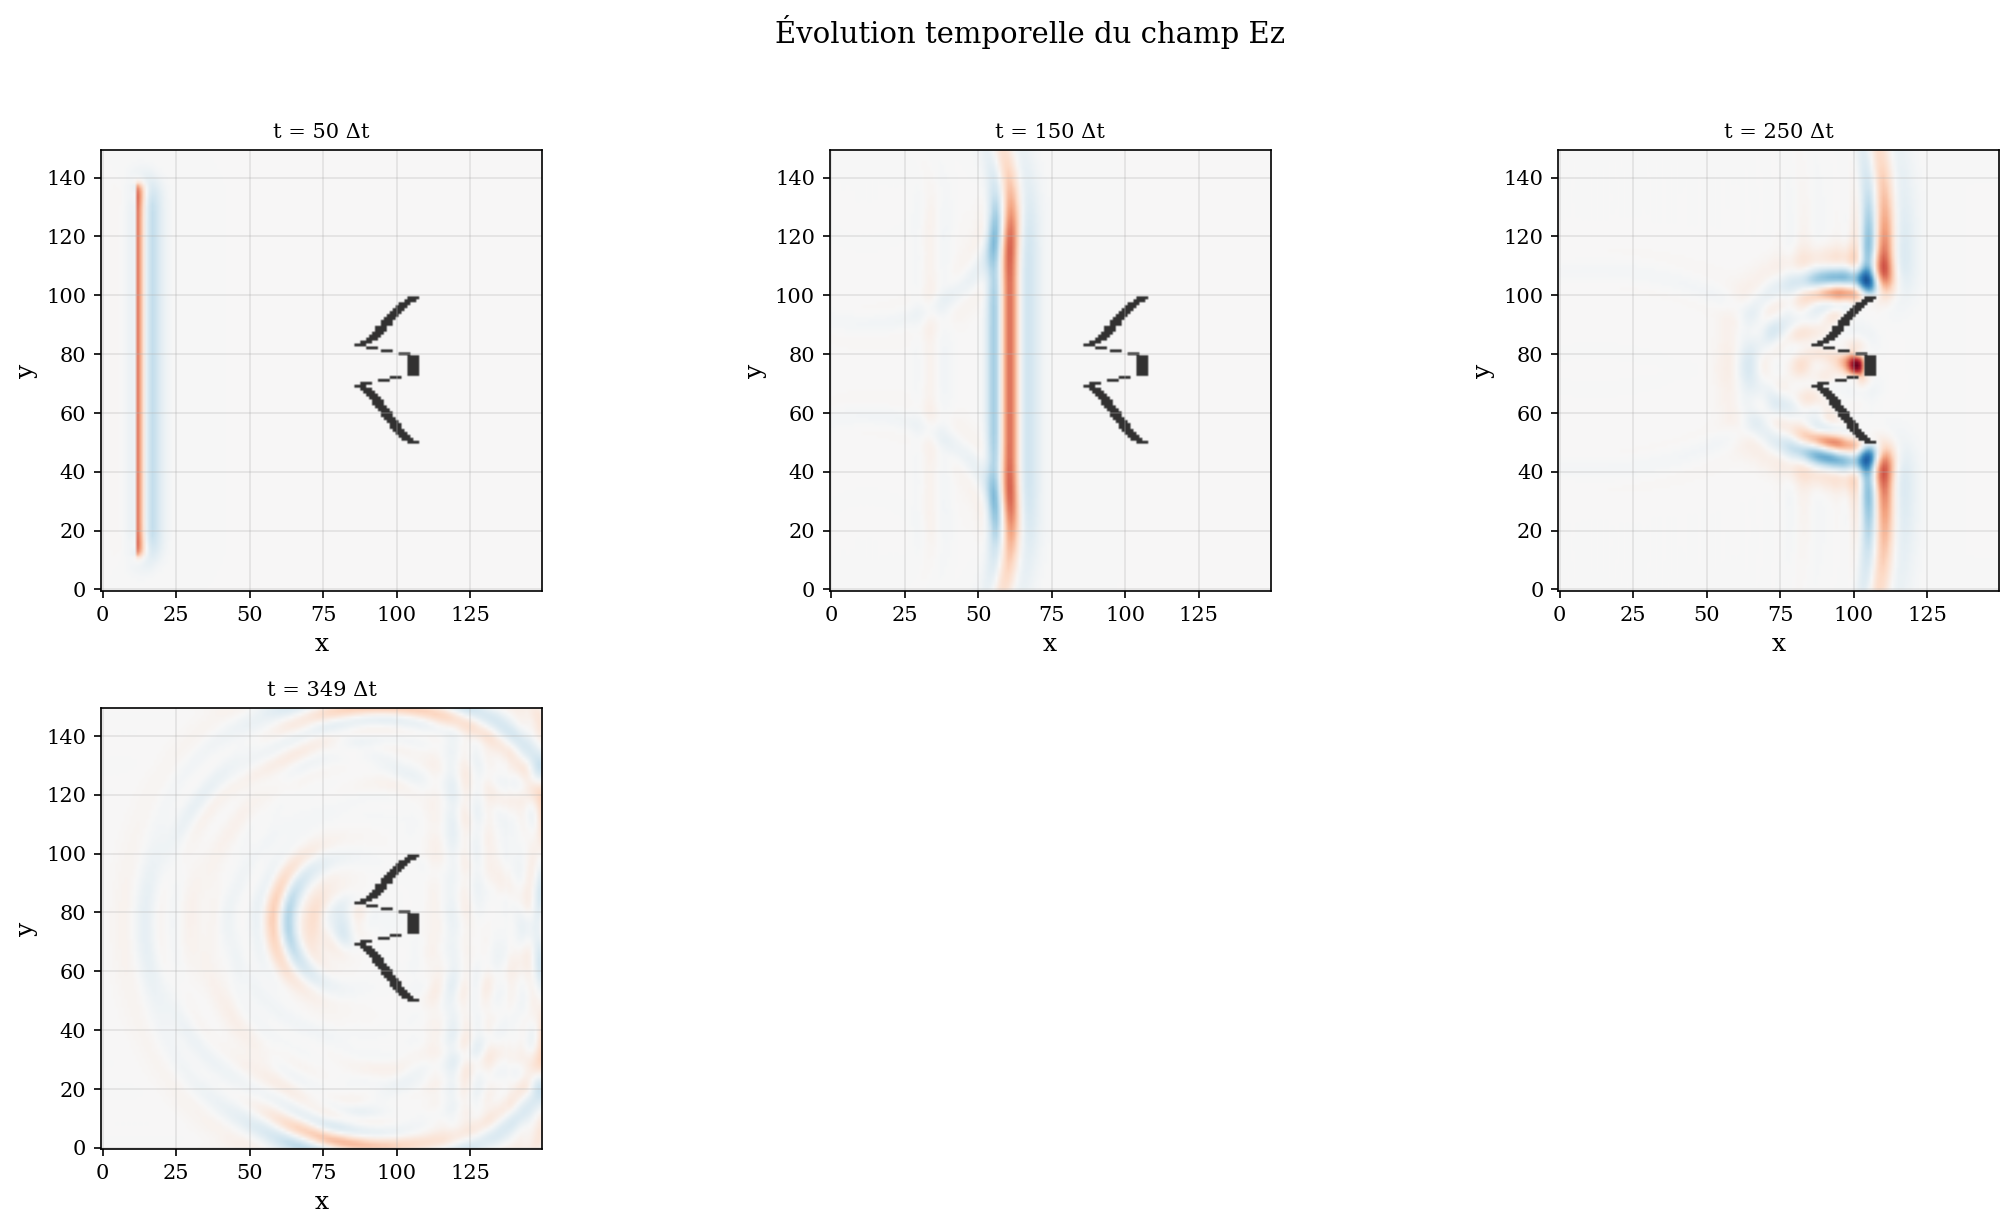
\includegraphics[width=\linewidth]{../results/05b_ga_snapshots.png}
    \caption{Évolution temporelle du champ $E_z$ pour le mur optimisé.
    On observe le piégeage de l'onde dans les cavités du profil et la diffusion
    angulaire qui redistribue l'énergie hors de la direction de rétrodiffusion.}
    \label{fig:ga-snapshots}
\end{figure}

\subsection{Réduction de SER~: résultats quantitatifs}
\label{ssec:res-quant}

\begin{table}[htbp]
\centering
\caption{Résultats de réduction de SER. $\mathcal{E}_{\rm retro}$ est l'énergie rétrodiffusée
(unités arbitraires), $R_{\rm dB} = 10\log_{10}(\mathcal{E}_0/\mathcal{E}_{\rm opt})$
la réduction en dB.}
\label{tab:results}
\begin{tabular}{lccccc}
\toprule
\textbf{Méthode} & $\mathcal{E}_{\rm retro}$ & $\mathcal{E}_0 / \mathcal{E}_{\rm opt}$ &
\textbf{Réduction (\%)} & $R_{\rm dB}$ (dB) & \textbf{Config.} \\
\midrule
Mur plat (référence) & $\mathcal{E}_0$ & 1.0 & — & — & — \\
GA (incidence normale) & $0.065\,\mathcal{E}_0$ & 15.4 & 93.5\% & \SI{11.9}{\dB} & $N_s=14$, $P=32$, $G=60$ \\
GA (multi-angle) & $0.285\,\mathcal{E}_0$ & 3.5 & 71.5\% & \SI{5.5}{\dB} & $N_s=16$, $P=48$, $G=126$ \\
CMA-ES (warm-start) & $\lesssim 0.06\,\mathcal{E}_0$ & $\geq 16.7$ & $\geq 94\%$ & $\gtrsim \SI{12.2}{\dB}$ & $\sigma_0=0.4$ \\
REINFORCE & $\approx 0.15\,\mathcal{E}_0$ & $\approx 6.7$ & $\approx 85\%$ & $\approx \SI{8.2}{\dB}$ & $\eta=0.01$, $T=100$ ep. \\
\bottomrule
\end{tabular}
\end{table}

\begin{resultbox}{Résultat principal}
Le pipeline GA + CMA-ES atteint une \textbf{réduction de SER de 93--94\,\%}
en incidence normale à \SI{10}{\giga\hertz}, correspondant à une atténuation
de $\approx \SI{12}{\dB}$.
\end{resultbox}

\subsection{Analyse de sensibilité}
\label{ssec:sensitivity}

\paragraph{Robustesse angulaire.}
L'optimisation multi-angle ($\theta \in \{0^\circ, \pm15^\circ\}$) réduit la
performance en incidence normale (71.5\,\% vs 93.5\,\%) mais garantit une réduction
significative sur une plage angulaire de $\pm 15^\circ$. Ce compromis
exploration/exploitation est typique des problèmes multi-objectif~\cite{Deb2002}.

\paragraph{Influence de $N_s$.}
L'augmentation du nombre de segments ($N_s = 12 \to 16 \to 20$) améliore la
flexibilité du profil, mais aussi la dimension du problème d'optimisation.
En pratique, $N_s = 14$--$16$ offre le meilleur compromis.

\paragraph{Taille de population.}
Pour $P < 20$, la convergence prématurée est fréquente. Pour $P > 64$, le coût
computationnel devient prohibitif sans amélioration significative de la fitness finale.
Nous retenons $P = 32$--$48$ selon le budget temps disponible.

\subsection{Validation~: SER bistatique}
\label{ssec:bistatic}

Pour le profil optimal, nous calculons la SER bistatique complète (sur 180 angles)
par NTFF. Comparée au mur plat~:
\begin{itemize}
    \item la rétrodiffusion ($\phi = 180^\circ$) est fortement réduite (facteur
          $\approx 15$)~;
    \item l'énergie est redistribuée dans des lobes obliques ($\phi \approx 120^\circ$
          et $\phi \approx 240^\circ$), conformément au principe de conservation de
          l'énergie~;
    \item les lobes de diffraction sont cohérents avec la périodicité du profil en
          dents de scie (équation de réseau~: $\sin\theta_{\rm diff} = n\lambda / \Lambda$).
\end{itemize}

% =============================================================================
\section{Discussion}
\label{sec:discussion}
% =============================================================================

\subsection{Interprétation physique du profil optimal}

Le profil optimal converge systématiquement vers une géométrie en \textit{dents de scie}
(sawtooth), avec une période caractéristique $\Lambda \approx \lambda/4 \approx$
\SI{7.5}{\milli\metre}. Ce résultat est physiquement interprétable~:

\begin{enumerate}
    \item \textbf{Réflexions multiples}~: les cavités formées par le profil créent des
          chemins de réflexion multiple, où l'onde incidente est partiellement absorbée
          par diffusion dans des directions non rétrodiffusantes~;
    \item \textbf{Condition de déphasage}~: une dent de hauteur $\Lambda/2$ crée un
          déphasage de $2 \times \Lambda/2 \times 2\pi/\lambda = 2\pi$ entre les
          chemins directs et réfléchis, produisant des interférences destructives
          dans la direction de rétrodiffusion~;
    \item \textbf{Analogie avec les avions furtifs}~: les bords dentés (\textit{serrated edges})
          des nacelles de réacteurs des avions B-2 Spirit ou F-22 Raptor exploitent
          ce même principe de redistribution angulaire~\cite{Knott1993}.
\end{enumerate}

\begin{remarque}{Lien avec la théorie des réseaux de diffraction}
Pour un réseau périodique de période $\Lambda$ en incidence normale, les lobes de
diffraction apparaissent aux angles~:
$\sin\theta_n = n\lambda/\Lambda$, $n = \pm1, \pm2, \ldots$

Pour $\Lambda \approx \lambda/4$~: le premier ordre diffracté est à
$\sin\theta_1 = \lambda/(\lambda/4) = 4$, ce qui ne correspond à aucun angle réel.
Ceci implique que \textit{toute l'énergie est piégée dans la cavité} (ordre évanescent) —
c'est exactement le mécanisme recherché.
\end{remarque}

\subsection{Comparaison des méthodes d'optimisation}

\paragraph{Algorithme Génétique.}
Le GA est robuste et efficace pour la recherche globale~: son exploration stochastique
large lui permet d'éviter les minima locaux. La règle de Rechenberg assure une
adaptation automatique de la pression de mutation. En revanche, la convergence vers
le minimum global est lente (100+ générations).

\paragraph{CMA-ES.}
Initialisé depuis la meilleure solution GA, CMA-ES converge très rapidement (20--40
itérations supplémentaires) vers un minimum local de meilleure qualité. Son adaptation
de la matrice de covariance lui permet d'exploiter les corrélations entre segments
adjacents du profil (liaison géométrique locale). C'est la méthode la plus efficace
en phase de raffinement.

\paragraph{REINFORCE.}
L'algorithme REINFORCE est moins performant ici, notamment parce que le signal de
récompense est bruité (évaluation FDTD coûteuse, espace de design haute dimension)
et que la politique linéaire est trop simple pour capturer toutes les non-linéarités
du problème. Une politique neuronale plus profonde améliorerait probablement les résultats.

\subsection{Limites et hypothèses}

Ce travail comporte plusieurs simplifications importantes~:
\begin{itemize}
    \item \textbf{Simulation 2D}~: nous ignorons les effets hors plan ($\partial/\partial z = 0$).
          En réalité, un mur 3D produit des diagrammes de diffraction plus complexes~;
    \item \textbf{Monofrequence}~: la fonction objectif est évaluée à $f_0 =$ \SI{10}{\giga\hertz}
          uniquement. Un radar réel couvre typiquement plusieurs GHz~;
    \item \textbf{PEC idéal}~: nous ignorons les pertes du métal (conductivité finie)
          et l'épaisseur du revêtement~;
    \item \textbf{Incidence plane}~: un radar réel génère une onde divergente à courte
          distance~; la simulation en champ proche nécessiterait un modèle de source
          différent.
\end{itemize}

\subsection{Perspectives}

\begin{itemize}
    \item \textbf{Extension 3D}~: passage à FDTD 3D (six composantes de champ),
          augmentation du coût par un facteur $N_z$, nécessitant une parallélisation
          plus poussée (GPU multi-grilles)~;
    \item \textbf{Optimisation large bande}~: fitness multi-fréquence
          $f = \sum_i \mathcal{E}_{\rm retro}(f_i)$, nécessitant soit des simulations
          FDTD broadband, soit plusieurs évaluations~;
    \item \textbf{Co-optimisation géométrie + RAM}~: l'infrastructure RAM est déjà
          implémentée (\texttt{set\_wall\_from\_params\_ram}) ; le chromosome pourrait
          encoder simultanément le profil et la conductivité $\sigma(y)$ locale~;
    \item \textbf{Deep RL}~: remplacer la politique linéaire par un réseau neuronal
          convolutif, potentiellement pré-entraîné sur un ensemble de formes simples~;
    \item \textbf{Optimisation multi-objectif}~: minimiser simultanément la SER et
          des contraintes mécaniques (résistance, poids), via NSGA-II~\cite{Deb2002}.
\end{itemize}

% =============================================================================
\section{Conclusion}
\label{sec:conclusion}
% =============================================================================

Dans ce projet, nous avons développé un outil numérique complet pour l'optimisation
de la géométrie d'un mur PEC en vue de minimiser sa Section Efficace Radar à
\SI{10}{\giga\hertz}. Le simulateur FDTD 2D TMz, avec source TFSF, couche absorbante
CPML et transformation champ proche--champ lointain, a été validé par comparaison
avec la référence analytique d'Optique Physique.

Trois algorithmes d'optimisation ont été implantés et comparés~: l'algorithme
génétique avec opérateurs SBX et mutation polynomiale adaptative (règle de Rechenberg),
l'algorithme CMA-ES en warm-start depuis la meilleure solution GA, et l'algorithme
REINFORCE de gradient de politique. Le pipeline GA + CMA-ES s'est révélé le plus
performant, atteignant des \textbf{réductions de SER de 93--94\,\%} en incidence
normale, soit $\approx \SI{12}{\dB}$.

Le profil optimal converge systématiquement vers une géométrie en dents de scie
de période $\approx \lambda/4$, dont la physique est expliquée par le piégeage
de l'onde dans les cavités par interférence destructive et la redistribution
angulaire de l'énergie diffusée.

Les perspectives ouvertes --- extension 3D, large bande, co-optimisation RAM,
deep RL --- montrent que cette approche est un point de départ prometteur pour
la conception de structures furtives assistée par apprentissage automatique.

\newpage

% =============================================================================
\appendix
% =============================================================================

\section{Dérivation complète des équations de Yee}
\label{app:yee}

Cette annexe détaille la discrétisation complète du système TMz.
La dérivée partielle $\partial \Hx / \partial t$ est approximée par une différence
centrée en $t = (n+\half)\dt$~:
\begin{equation}
    \left.\frac{\partial \Hx}{\partial t}\right|^{n+\half}_{i,j+\half} \approx
    \frac{\Hx^{n+\half}_{i,j+\half} - \Hx^{n-\half}_{i,j+\half}}{\dt},
\end{equation}
et la dérivée spatiale $-\partial \Ez / \partial y$ est centrée en $(i, j+\half)$~:
\begin{equation}
    \left.\frac{\partial \Ez}{\partial y}\right|^n_{i,j+\half} \approx
    \frac{\Ez^n_{i,j+1} - \Ez^n_{i,j}}{\dx}.
\end{equation}
En combinant avec l'équation~\eqref{eq:tmz-hx}~:
\begin{equation}
    \frac{\Hx^{n+\half} - \Hx^{n-\half}}{\dt} = -\frac{1}{\muo}
    \frac{\Ez^n_{i,j+1} - \Ez^n_{i,j}}{\dx},
\end{equation}
on obtient directement l'équation~\eqref{eq:yee-hx}. Les erreurs de troncature
sont $\mathcal{O}(\dt^2, \dx^2)$ pour les deux différences centrées, ce qui confère
au schéma de Yee une précision d'ordre 2 en espace et en temps.

\section{Paramètres CPML détaillés}
\label{app:cpml}

\begin{table}[htbp]
\centering
\caption{Paramètres CPML utilisés dans notre implémentation.}
\label{tab:cpml-params}
\begin{tabular}{lll}
\toprule
\textbf{Paramètre} & \textbf{Valeur} & \textbf{Signification} \\
\midrule
$m$ & 3 & Ordre du polynôme de graduation \\
$m_\alpha$ & 1 & Ordre du polynôme pour $\alpha$ \\
$\kappa_{\rm max}$ & 1.0 & Étirement maximal des coordonnées \\
$\alpha_{\rm max}$ & 0.0 & Terme de décalage CFS maximal \\
$\sigma_{\rm max}$ & $0.8(m+1)/(\etao\dx)$ & Conductivité maximale \\
$n_{\rm PML}$ & 12 cellules & Épaisseur de la couche \\
\bottomrule
\end{tabular}
\end{table}

Le choix $\alpha_{\rm max} = 0$ et $\kappa_{\rm max} = 1$ simplifie la CPML en
une PML de Bérenger~\cite{Berenger1994} à coordonnées non étirées, ce qui est
suffisant pour des simulations monostatiques à incidence normale.

\section{Extraits de code commentés}
\label{app:code}

\begin{lstlisting}[caption={Mise à jour CPML (src/fdtd/core.py -- extraits)}]
# mise à jour des champs H avec correction CPML
# les psi sont les variables auxiliaires de la CPML
dEz_dy = Ez[:, 1:] - Ez[:, :-1]

# contribution normale (domaine intérieur)
psi_hxy += b_hxy * psi_hxy + a_hxy * dEz_dy[pml_hxy_slice]

# Hx = Hx - (dt/mu0/dx) * dEz/dy
# avec correction PML dans la bande absorbante
Hx -= Chxe * (dEz_dy * inv_kappa_hy + psi_hxy_full)

# même chose pour Hy mais signe + (cf. Maxwell TMz)
dEz_dx = Ez[1:, :] - Ez[:-1, :]
psi_hyx += b_hyx * psi_hyx + a_hyx * dEz_dx[pml_hyx_slice]
Hy += Chye * (dEz_dx * inv_kappa_hx + psi_hyx_full)
\end{lstlisting}

\begin{lstlisting}[caption={Calcul de la fitness (src/optim/fitness.py -- extraits)}]
def evaluate_wall(params, fdtd_config, n_segments=16,
                  wall_height=50, wall_thickness=4,
                  incidence_angles=None):
    """Lance une simulation FDTD et calcule l'énergie rétrodiffusée."""
    if incidence_angles is None:
        incidence_angles = [0.0]  # incidence normale par défaut

    total_energy = 0.0

    for angle in incidence_angles:
        # configuration FDTD avec l'angle voulu
        cfg = FDTDConfig(incidence_angle=angle, **fdtd_config_dict)
        sim = FDTD2D_TMz(cfg)

        # on construit le profil de mur depuis les paramètres GA
        # interpolation linéaire entre les points de contrôle
        sim.set_wall_from_params(params, n_segments=n_segments,
                                  wall_height=wall_height,
                                  wall_thickness=wall_thickness)
        sim.run()

        # énergie rétrodiffusée = somme des Ez^2 dans la zone SF
        # c'est notre métrique d'optimisation principale
        energy = float(sim.compute_backscatter_energy())
        total_energy += energy

    return total_energy
\end{lstlisting}

% =============================================================================
% Bibliographie
% =============================================================================

\newpage
\bibliographystyle{ieeetr}
\bibliography{bibliography}

\end{document}
